\newpage
\section{Auswertung}
Im Folgenden werden die Ergebnisse der in Abschnitt \ref{sec:durchfuehrung} erläuterten Messungen mithilfe der Software \textit{MagicPlotStudent.exe} ausgewertet und die Ergebnisse dargestellt. \cite{magicplot}

\subsection{Abschätzung der Ausdehnung der Quantenpunkte}
\label{subsec:31}

In den Abbildungen \ref{fig:pl645} bis \ref{fig:pl520} sind die Photolumineszenzspektren der kolloidalen Quantenpunkte zu sehen. Dabei wurde bei der Probe mit der Emissionswellenlänge $\lambda_h=\SI{520}{\nano\meter}$ die Leistung
deutlich niedriger gewählt, als bei den anderen Proben um Sättigungseffekte im CCD-Chip zu vermeiden. Mithilfe der Formel \ref{eq: E_R} aus Kapitel \ref{sec:theo} wird die Ausdehnung $a_m$ bzw. $a_h$ der Quantenpunkte ermittelt. Mithilfe einer Ausgleichsrechnung an einer Normalverteilung wird die Halbwertsbreite $\Gamma_{\text{FWHM}}$ und die x-Position der Maxima $\lambda_m$ der PL-Intensität ermittelt. Die Ausdehnung wird je aus den Herstellerangaben $\lambda_h$ und aus den gemessenen Wellenlängen $\lambda_m$ berechnet. Die Ergebnisse sind in Tabelle \ref{tab:ausdehnung} zusammengestellt.
\begin{table}[H]
  \centering
  \caption{Mittels Ausgleichsrechnung ermittelte Halbwertsbreiten $\Gamma_{\text{FWHM}}$ und Wellenlängen $\lambda_m$, sowie die aus den Herstellerangaben $\lambda_h$ und gemessenen Wellenlängen $\lambda_m$ berechnete Ausdehnung $a_h$ bzw. $a_m$ der Quantenpunkte.}
  \label{tab:ausdehnung}
  \begin{tabular}{c|c|c|c|c}
    \toprule
    $\lambda_h$ in nm & $a_h$ in nm & $\lambda_m$ in nm & $a_m$ in nm & $\Gamma_{\text{FWHM}}$ in nm\\
    \midrule
    520 & 2.63 & $560.02 \pm 0.02$ & $3.1474 \pm 0.0003$ & $29.00 \pm 0.02$ \\
    580 & 3.51 & $588.72 \pm 0.04$ & $3.7022 \pm 0.0009$ & $36.27 \pm 0.04$ \\
    645 & 6.47 & $646.52 \pm 0.03$ & $ 6.651 \pm 0.004 $ & $33.44 \pm 0.04$ \\
    \bottomrule
  \end{tabular}
\end{table}
Die zur Berechnung der Ausdehnung verwendeten Materialparameter sind in Tabelle \ref{tab:const} gelistet. Dabei wurden die effektiven Massen der Ladungsträger und die Permittivität für eine Bewegung senkrecht zur ausgezeichneten Achse verwendet.
\begin{table}[H]
  \centering
  \caption{Zur Abschätzung der Ausdehnung benötigte Materialkonstanten. \cite{dissArens}}
  \label{tab:const}
  \begin{tabular}{c|c}
    \toprule
    $\epsilon_r $ & $ 9.15$ \\
    $m^*_h$ & $ -0.45 m_0$ \\
    $m^*_e $ & $ 0.15 m_0$ \\
    $E_g $ & $1.74\si{\electronvolt}$ \\
    \bottomrule
  \end{tabular}
\end{table}

Für die Proben mit $\lambda_h=\SI{580}{\nano\meter}$ und $\lambda_h=\SI{645}{\nano\meter}$ stimmen die Herstellerwerte mit den gemessenen Wellenlängen $\lambda_m$ überein, während der gemessene Wert zur $\lambda_h=\SI{520}{\nano\meter}$ stark abweicht.
Es ist deutlich zu sehen, dass die Größe der Quantenpunkte mit steigender Wellenlänge zunimmt. Anhand der Halbwertsbreiten der Photolumineszenzpeaks ist kein erkennbarer Trend feststellbar.
In Abbildung \ref{fig:pl645} und \ref{fig:pl580} ist außerdem eine Reflexion der Anregungswelle im Spektrum zu sehen.
Auffällig sind außerdem die in der $\lambda_h=\SI{645}{\nano\meter}$ auftretenden lokalen Maxima an der rechten Flanke des Emissionspeaks. Des Weiteren fällt an der abfallenden Flanke eine Schulter in den Messdaten der $\lambda_h=\SI{520}{\nano\meter}$ Probe auf.
Eine Abweichung der Gauß-Form des Lumnineszenzpeaks der $\lambda_h=\SI{580}{\nano\meter}$ Probe ist ebenfalls zu sehen.

\begin{figure}[H]
  \centering
  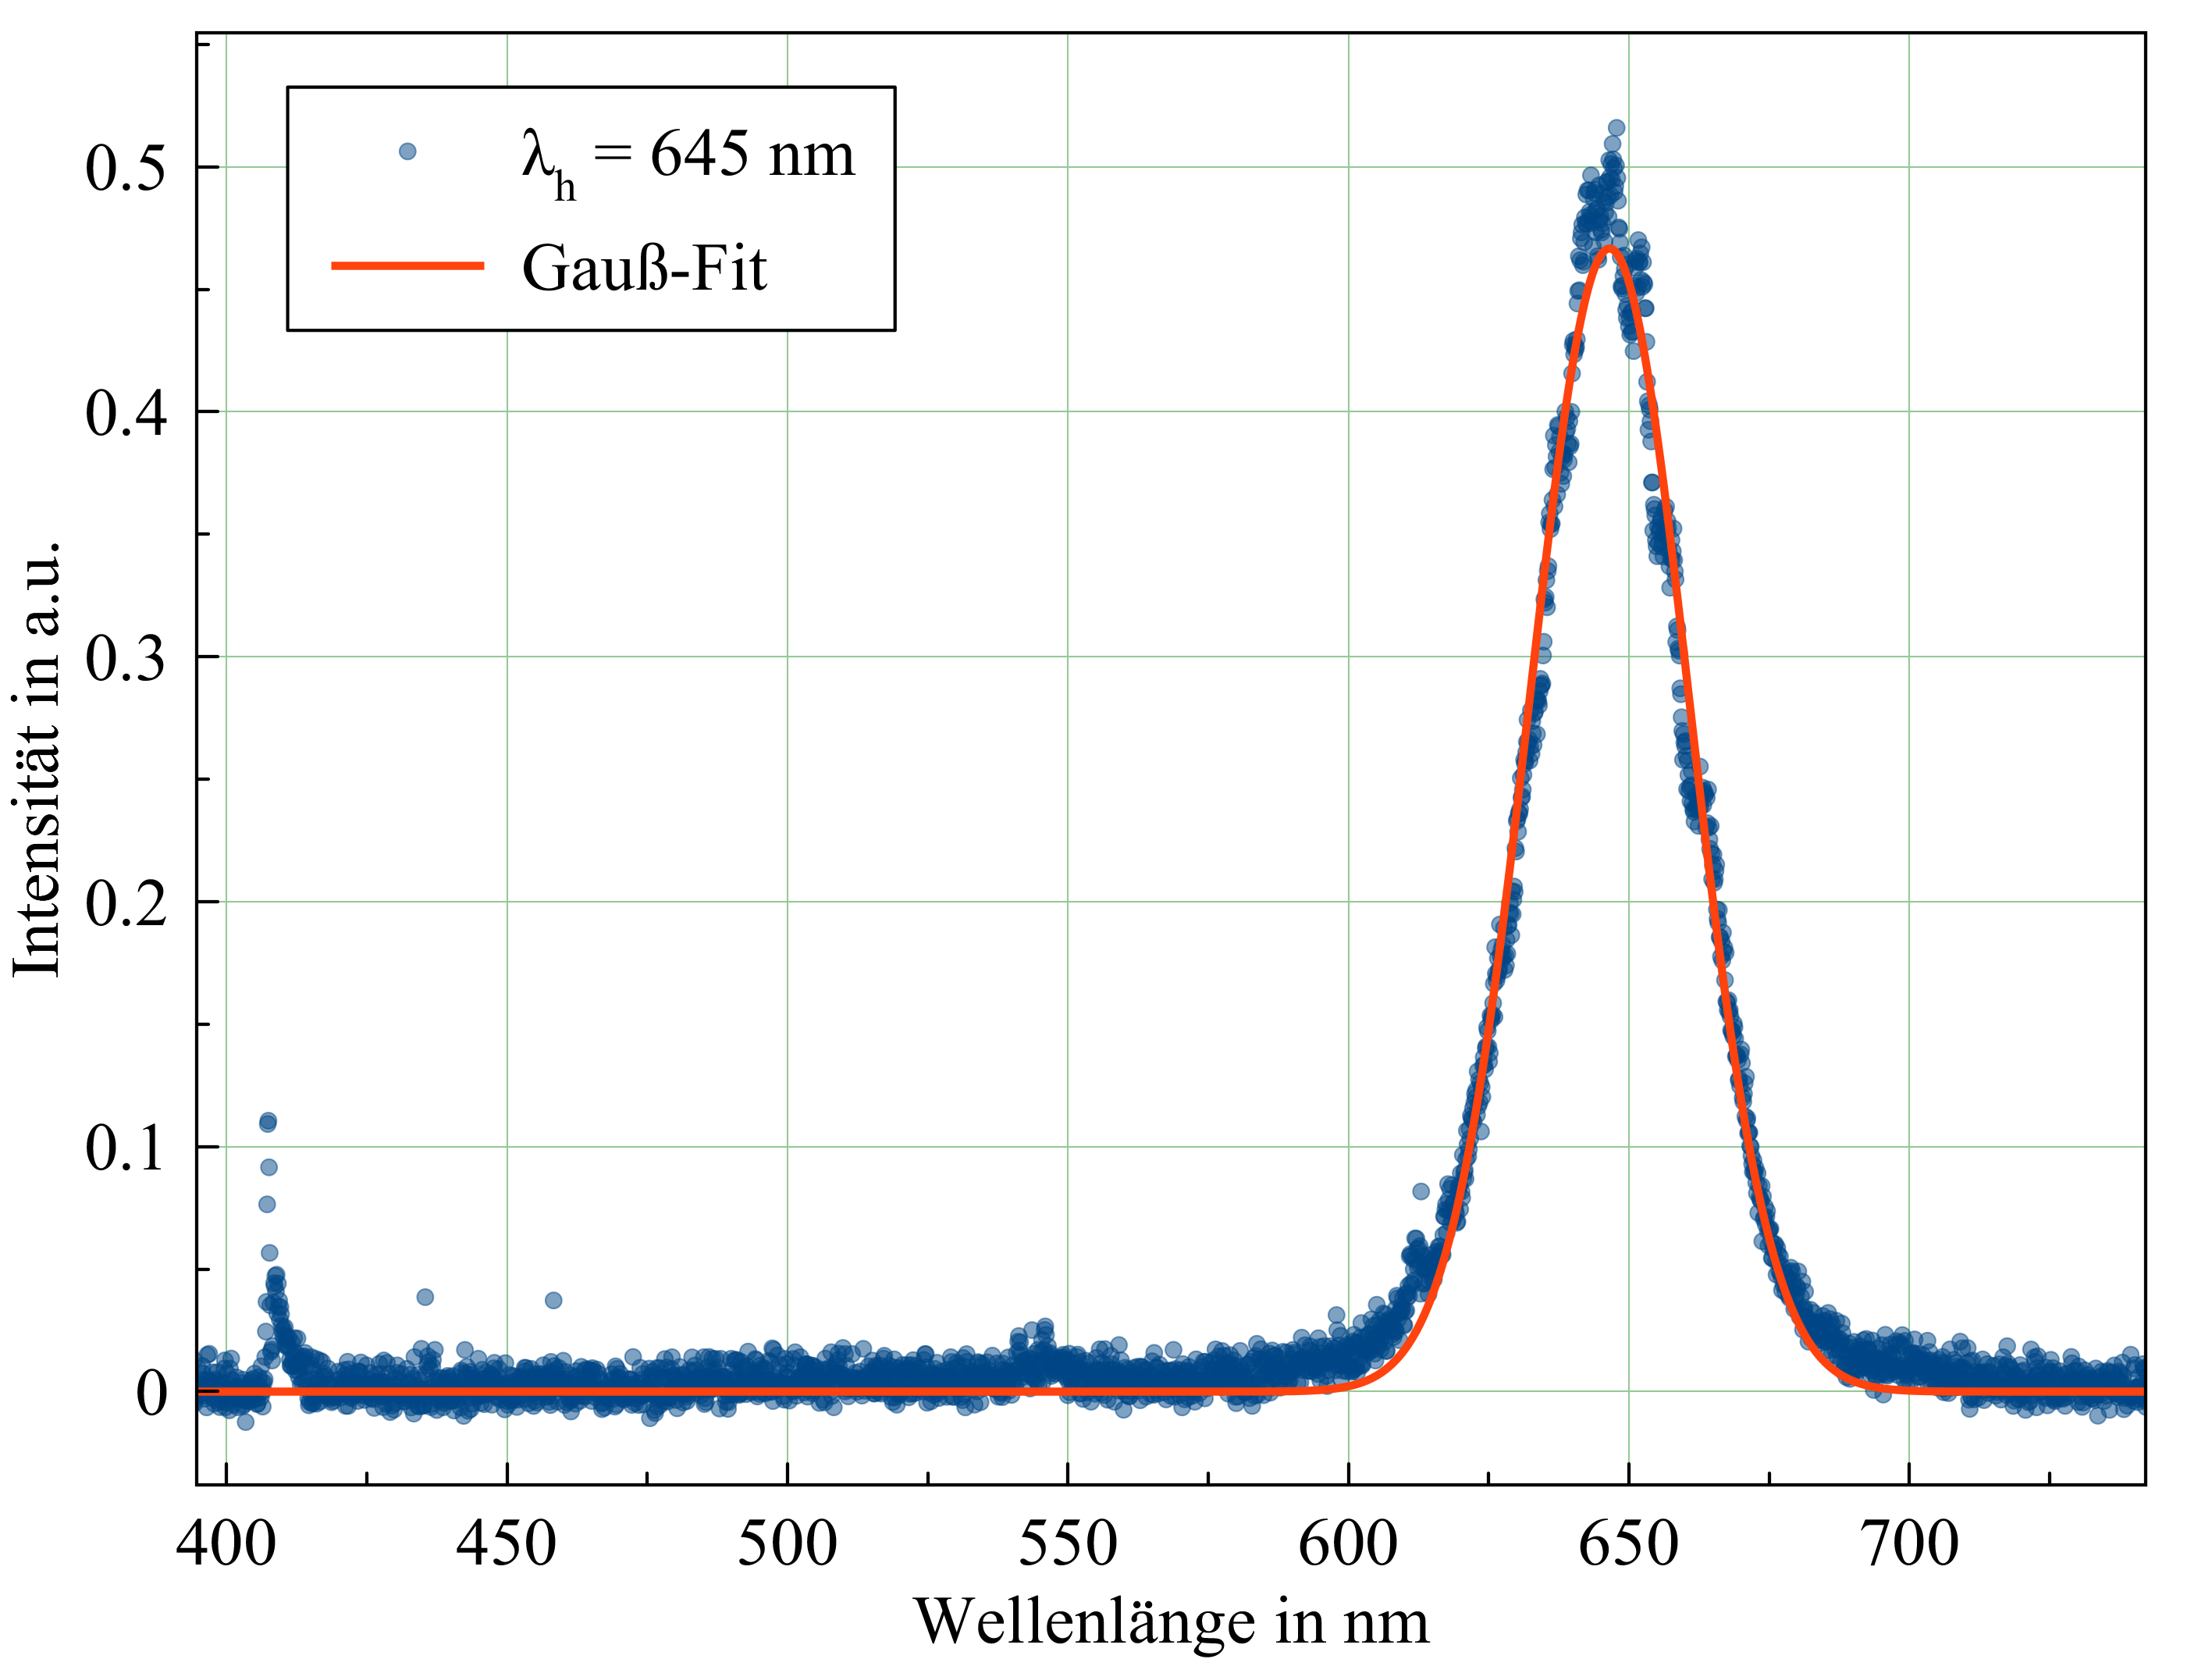
\includegraphics[width=0.7\textwidth]{plots/PL_645nm.png}
  \caption{Photolumineszenzspektrum einer Probe mit Emissionswellenlänge $\lambda_h=\SI{645}{\nano\meter}$ bei einer Anregungswellenlänge von $\lambda=\SI{405}{\nano\meter}$ und einer Eingangsleistung von $\SI{130}{\milli\watt}$.}
  \label{fig:pl645}
\end{figure}
\begin{figure}[H]
  \centering
  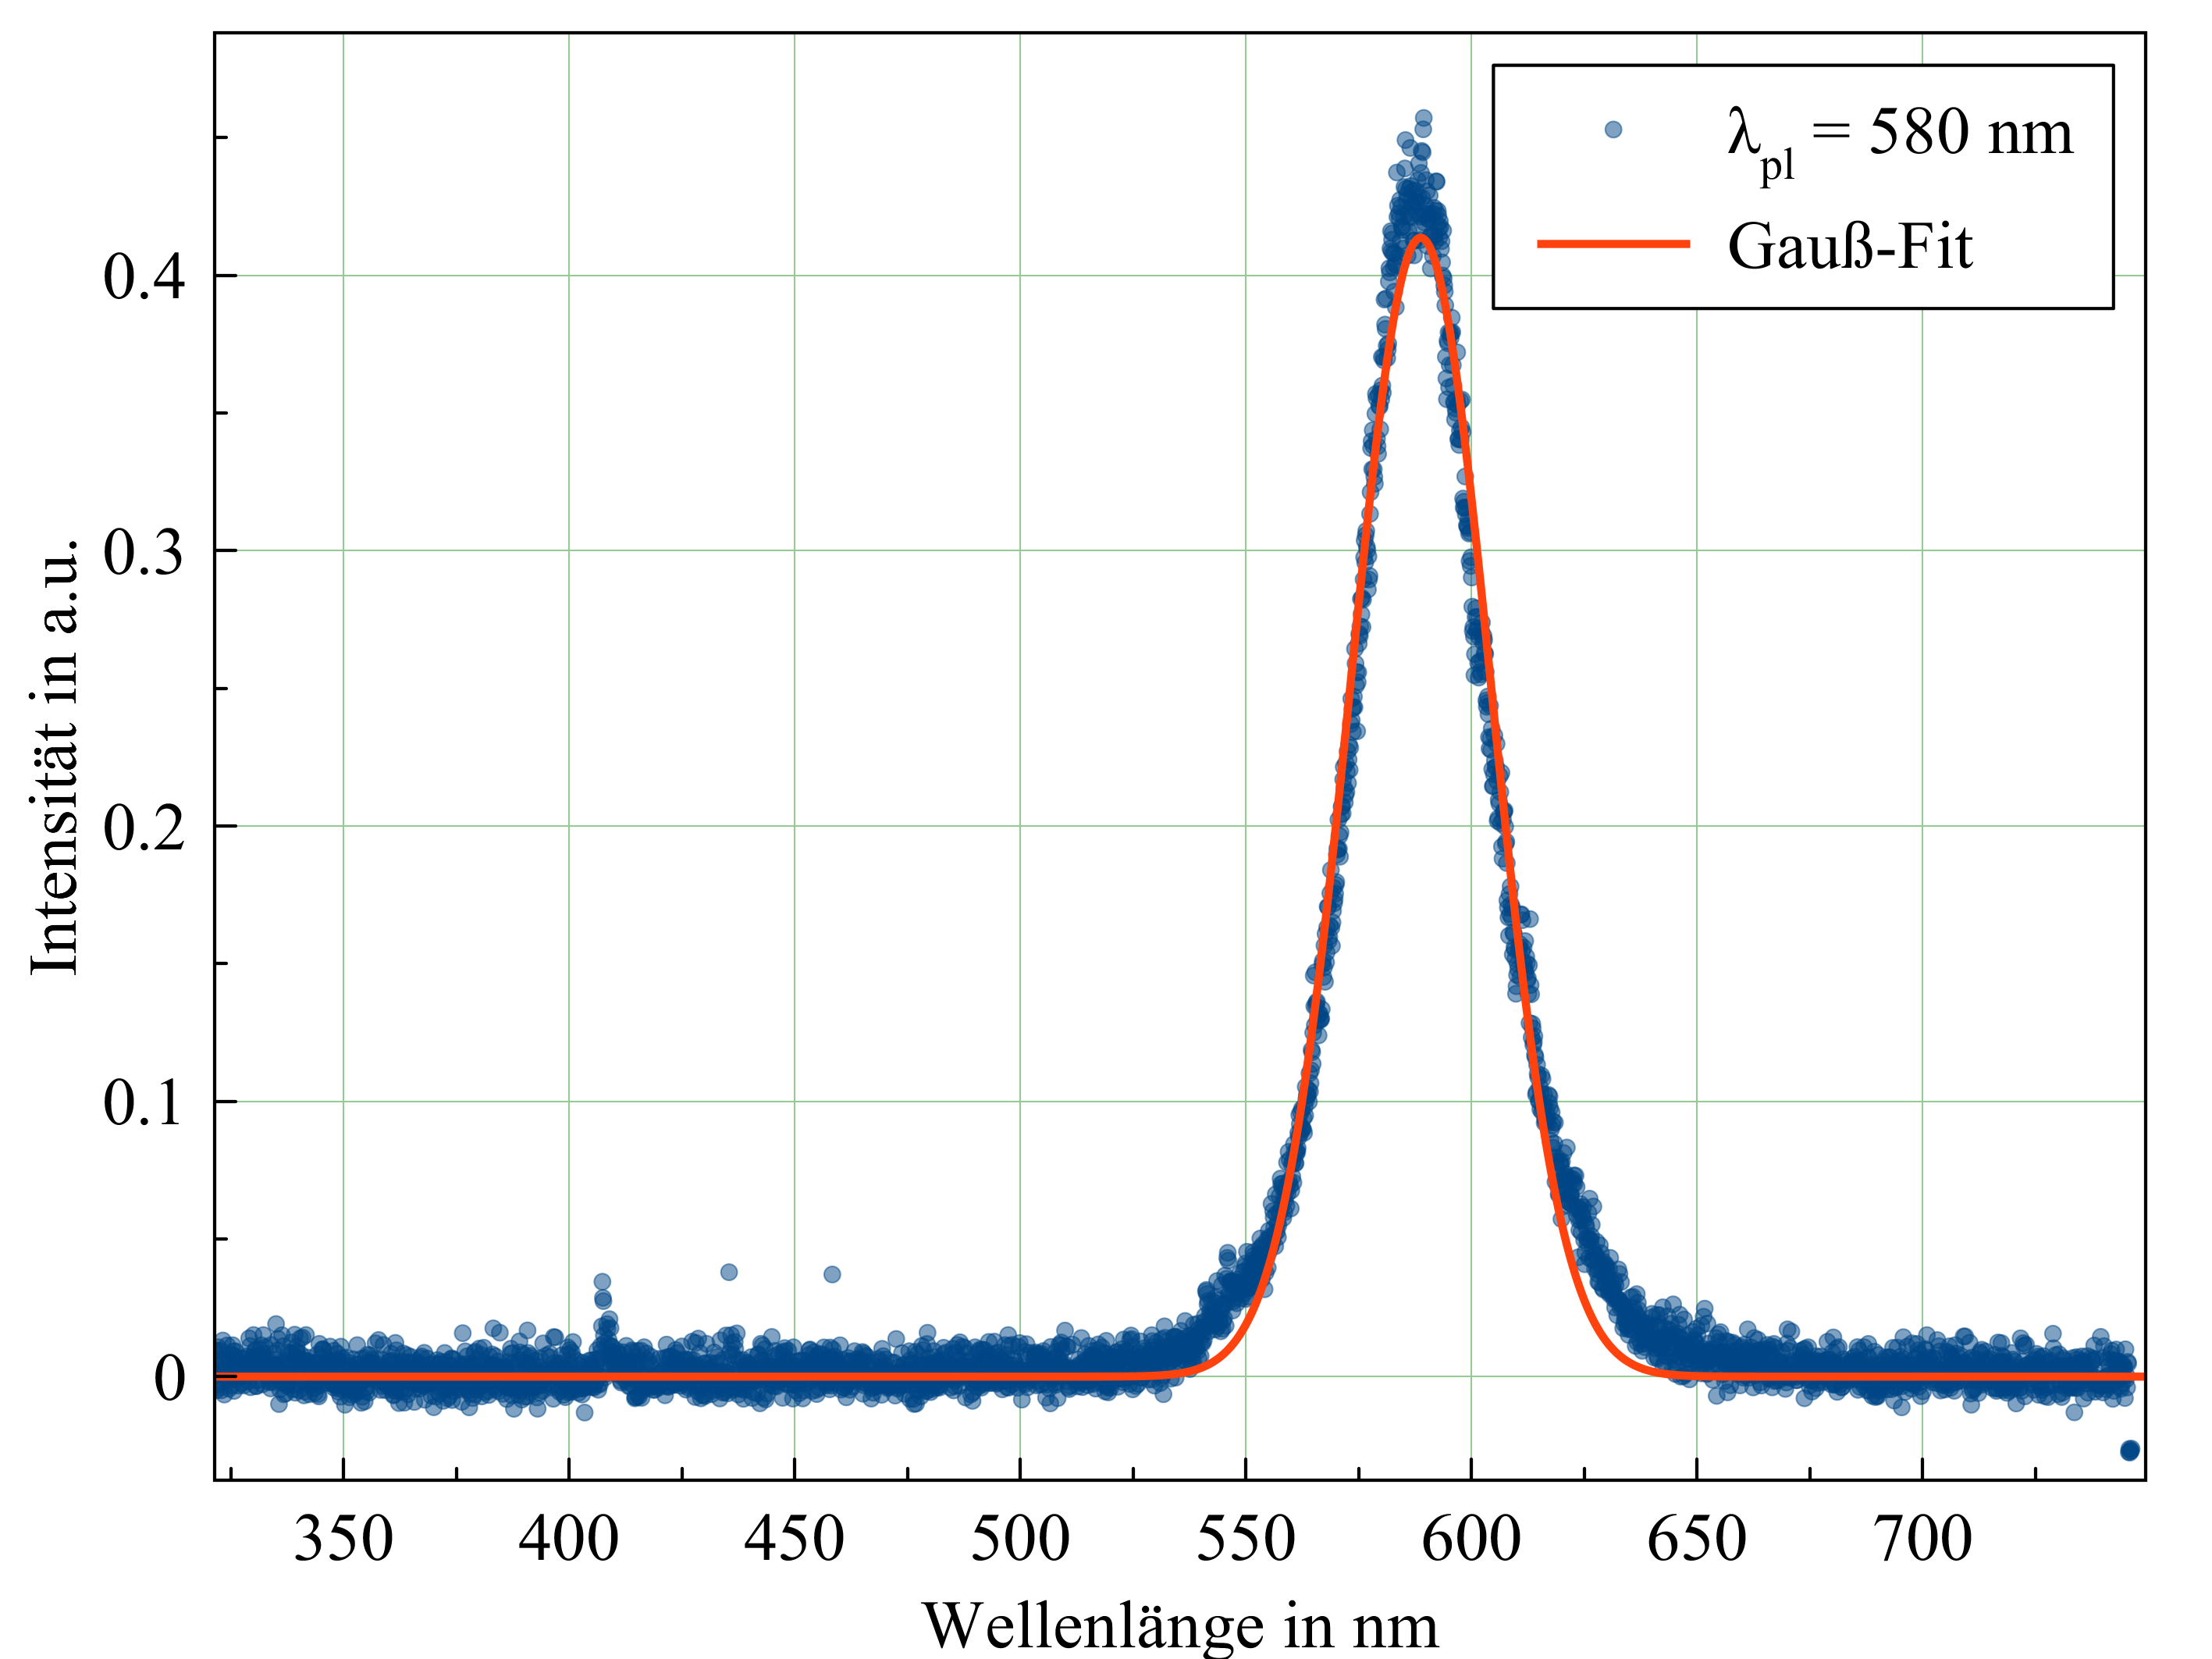
\includegraphics[width=0.7\textwidth]{plots/PL_580nm.png}
  \caption{Photolumineszenzspektrum einer Probe mit Emissionswellenlänge $\lambda_h=\SI{580}{\nano\meter}$ bei einer Anregungswellenlänge von $\lambda=\SI{405}{\nano\meter}$ und einer Eingangsleistung von $\SI{130}{\milli\watt}$.}
  \label{fig:pl580}
\end{figure}
\begin{figure}[H]
  \centering
  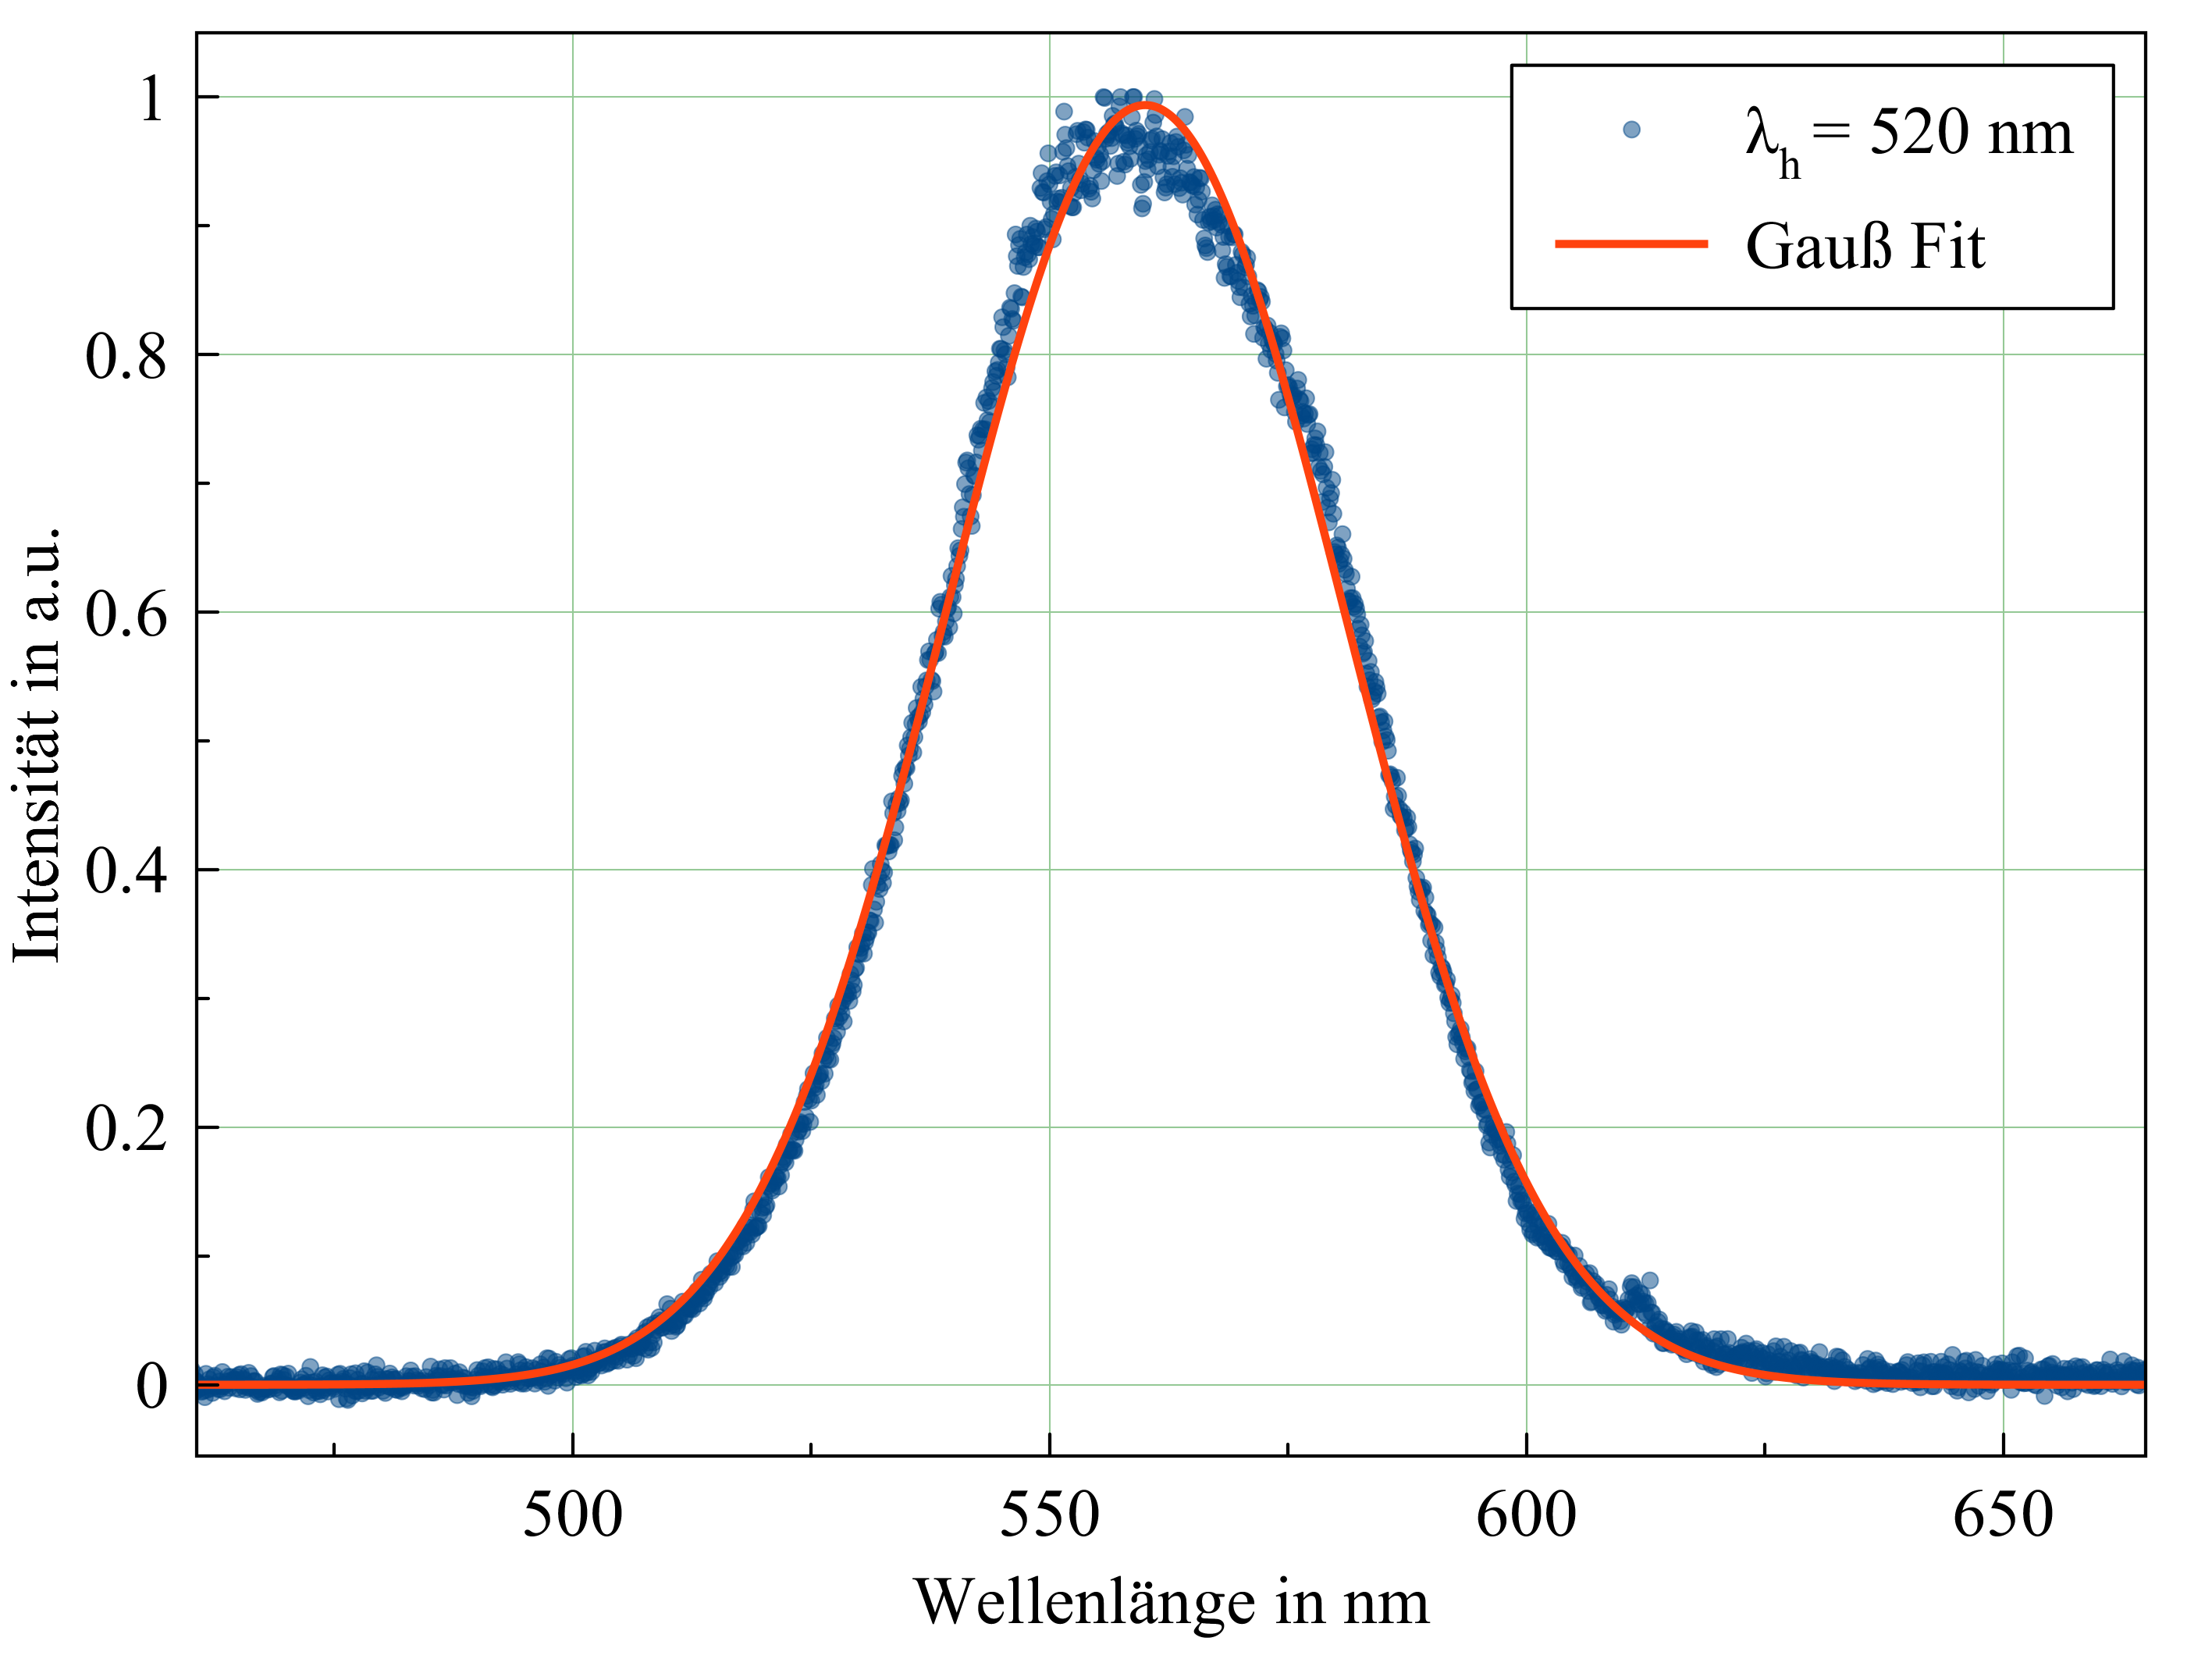
\includegraphics[width=0.7\textwidth]{plots/PL_520nm.png}
  \caption{Photolumineszenzspektrum einer Probe mit Emissionswellenlänge $\lambda_h=\SI{520}{\nano\meter}$ bei einer Anregungswellenlänge von $\lambda=\SI{405}{\nano\meter}$ und einer Eingangsleistung von $\SI{1,5}{\milli\watt}$.}
  \label{fig:pl520}
\end{figure}

\newpage
\subsection{Abhängigkeit der PL von der Eingangsleistung}
\label{sec:leistung}
Die Resultate der Untersuchung der Leistungsabhängigkeit sind in den Abbildungen ~\ref{fig:Podep520} und ~\ref{fig:Podep645} für zwei der Proben graphisch dargestellt.
Es ist zunächst ein linearer Anstieg zu sehen, welcher in eine Sättigung bei höheren Eingangsleistungen
übergeht. Der untersuchte Bereich der Leistung ist für die in Abbildung \ref{fig:Podep520} gezeigte Probe deutlich
kleiner, da der CCD-Chip eher in Sättigung geht.
\begin{figure}[H]
  \centering
  \begin{subfigure}{0.5\textwidth}
    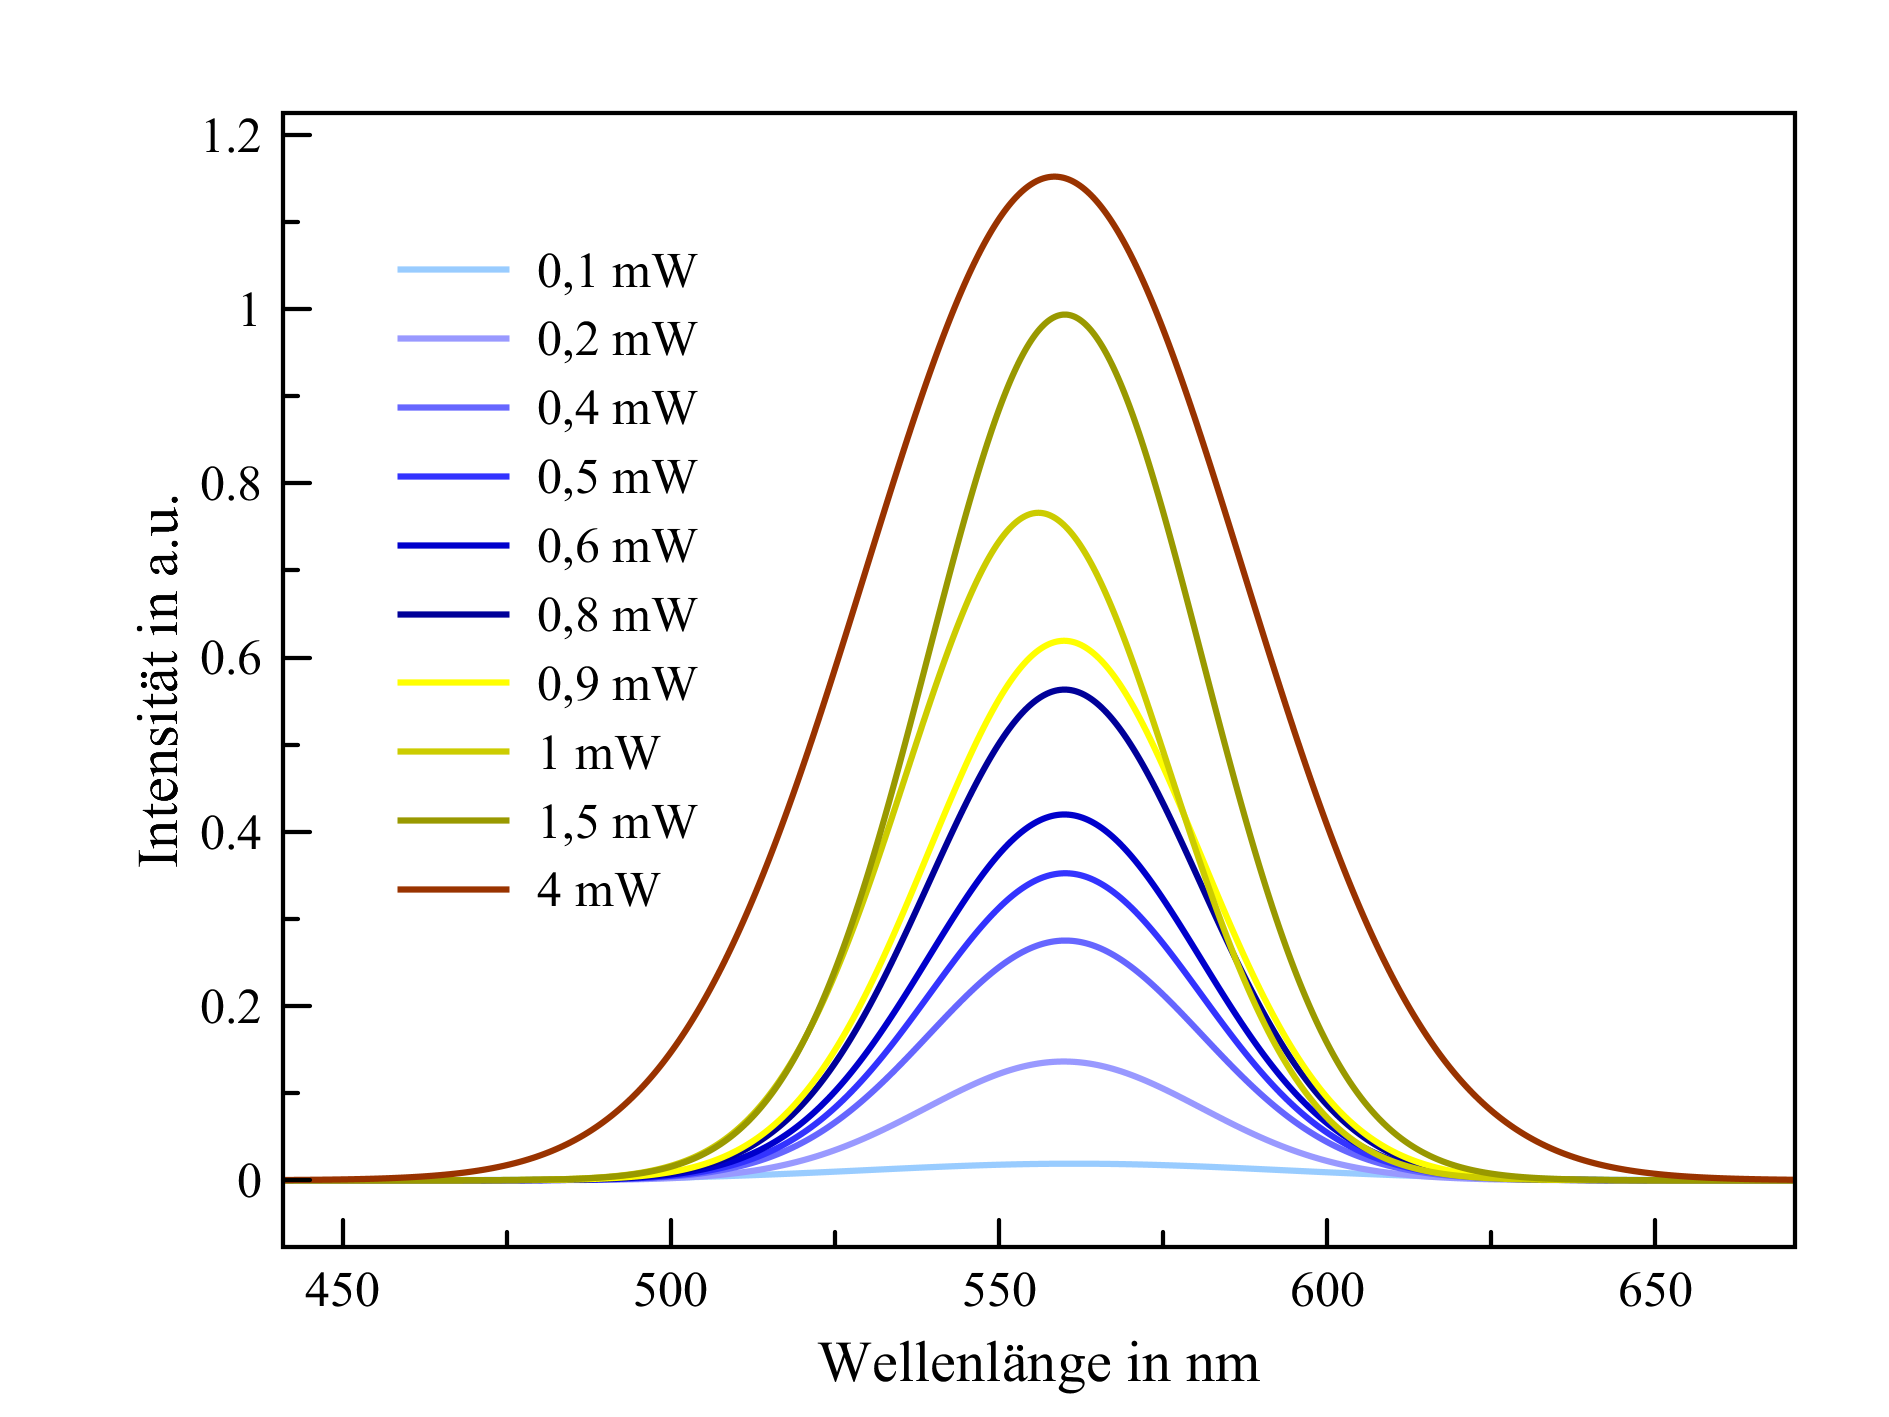
\includegraphics[width=\textwidth]{plots/Powerdependence_520nm.png}
  \end{subfigure}
  \begin{subfigure}{0.45\textwidth}
    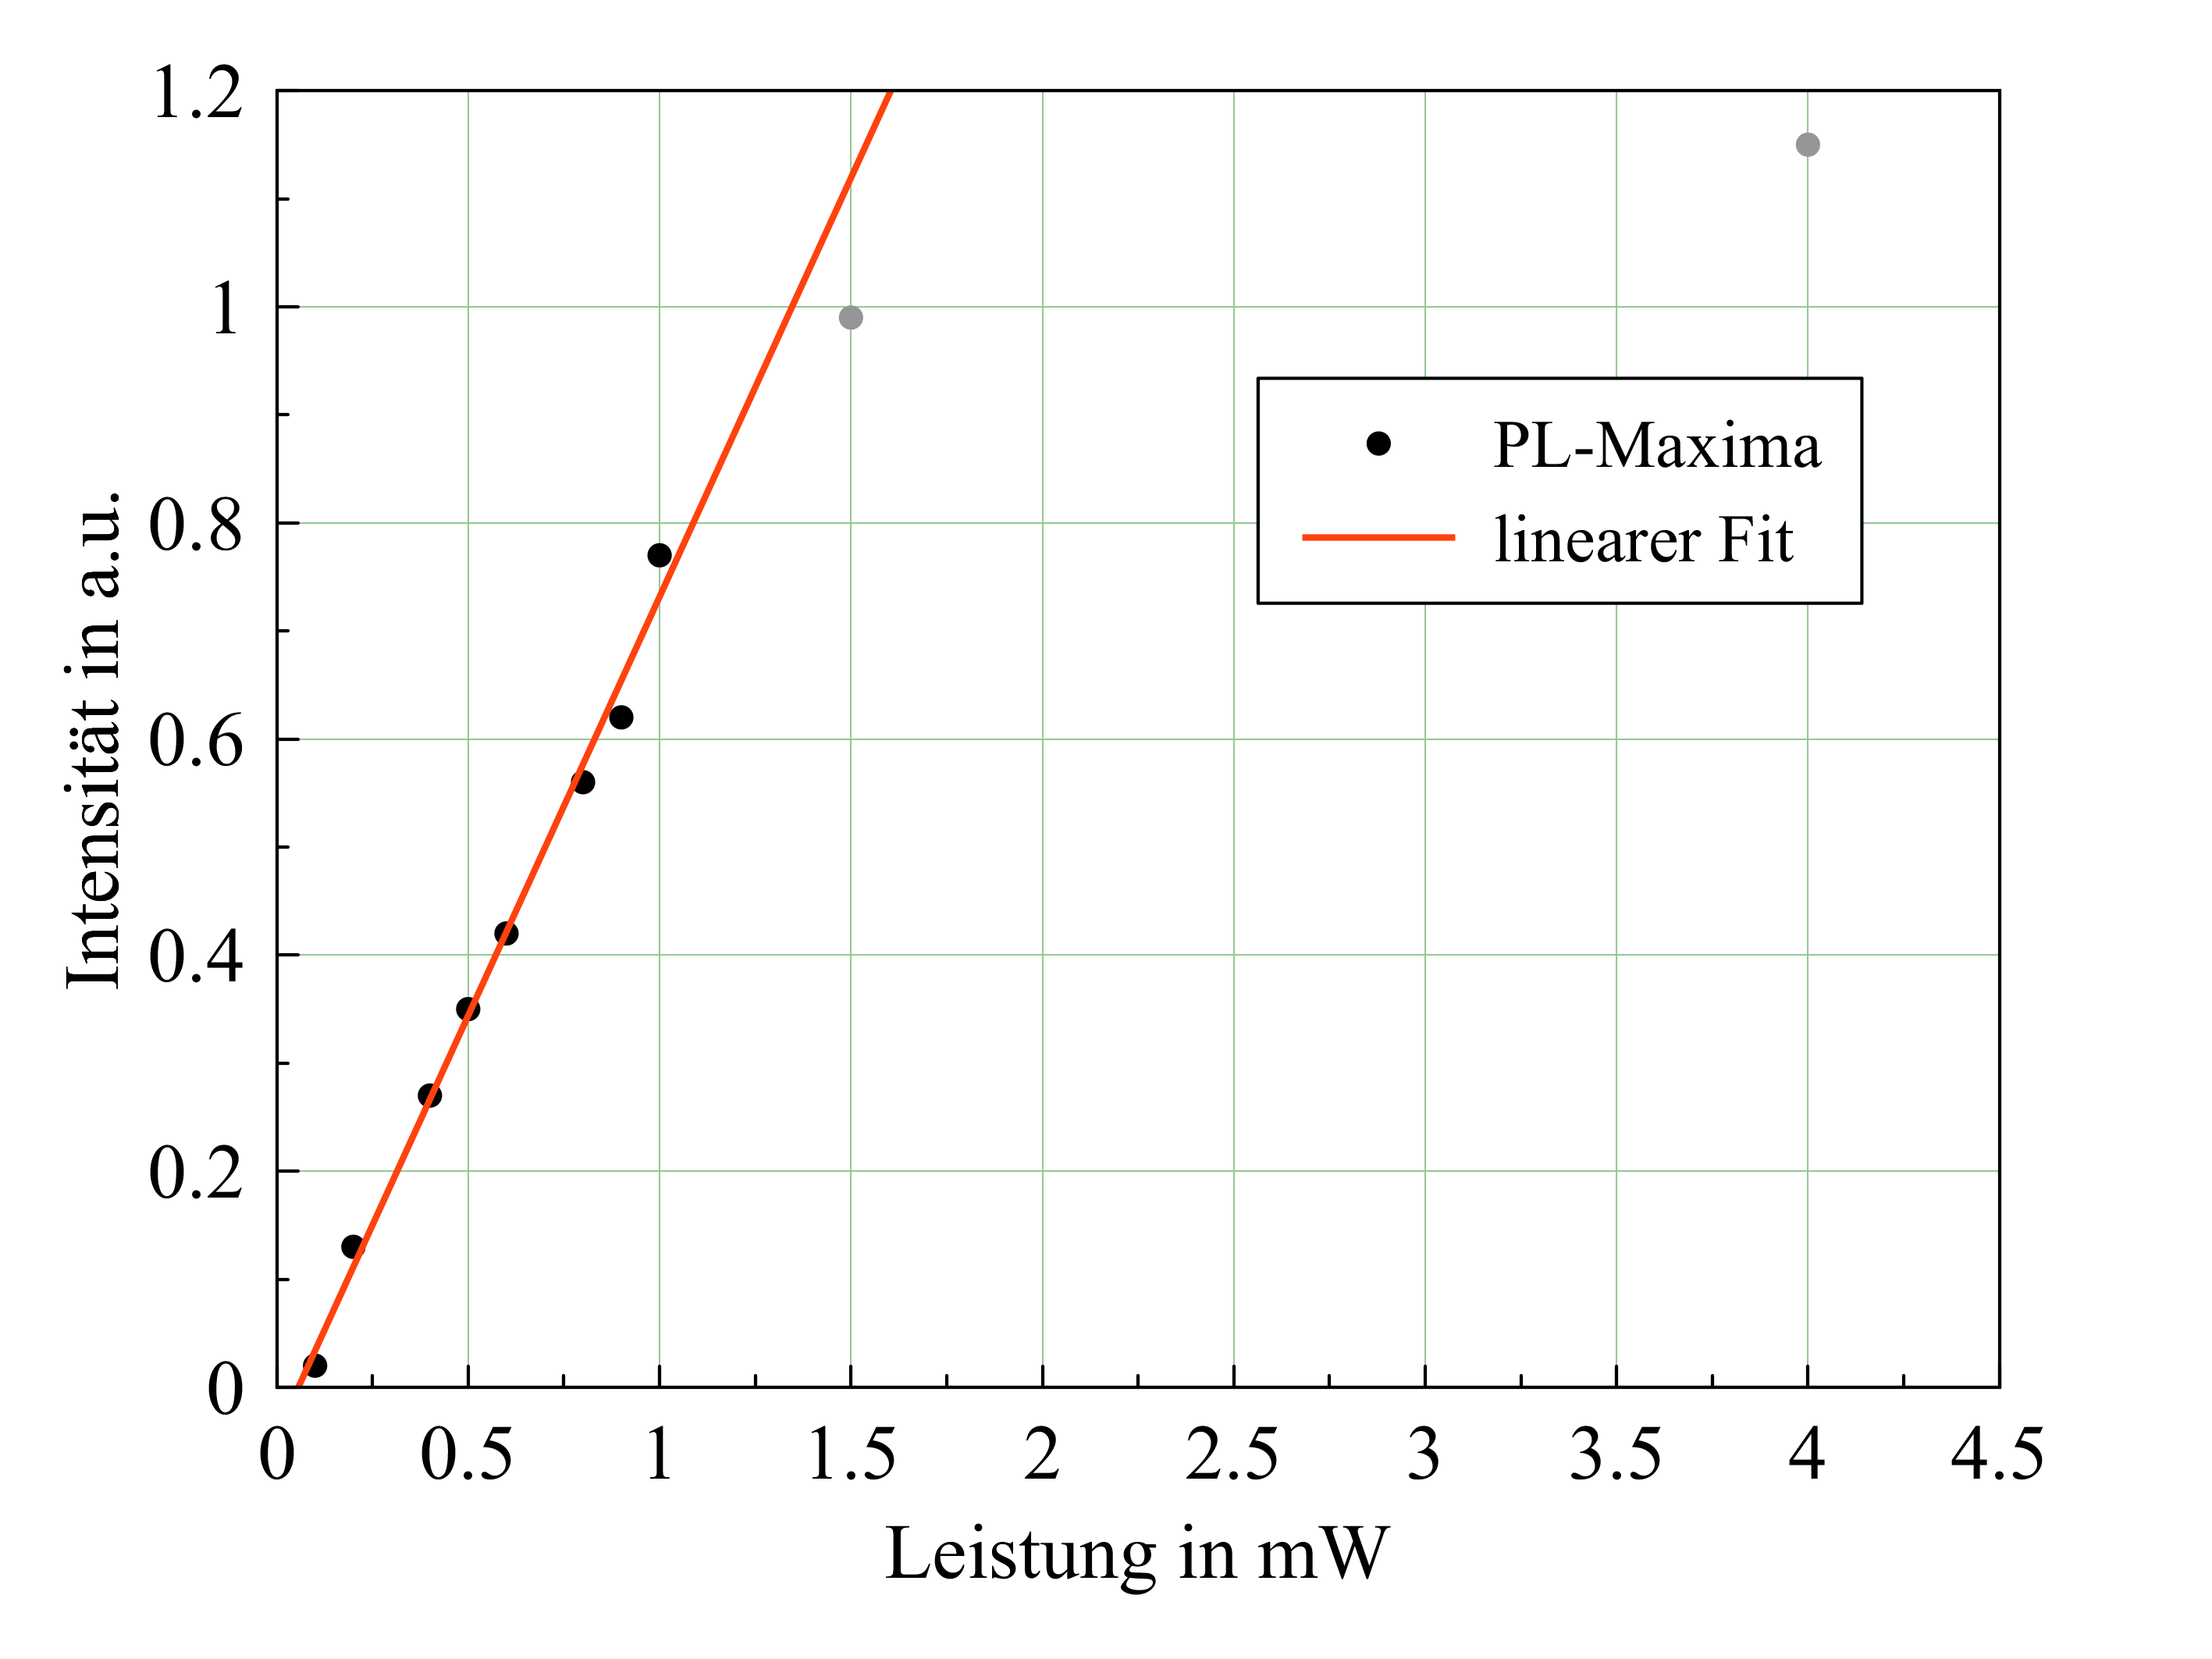
\includegraphics[width=\textwidth]{plots/Powerdepfit_520.png}
  \end{subfigure}
  \caption{Abhängigkeit der Photolumineszenz von der Eingangsleistung für eine Probe mit PL-Wellenlänge $\lambda_h = \SI{520}{\nano\meter}$.
  \textbf{Links:} Kurvenschar der Ausgleichsrechnungen der PL-Spektren für unterschiedliche Leistungen. \textbf{Rechts:} Darstellung der Maxima der Ausgleichskurven und Fit des linearen Anstiegs.}
  \label{fig:Podep520}
\end{figure}
\begin{figure}[H]
  \centering
  \begin{subfigure}{0.49\textwidth}
    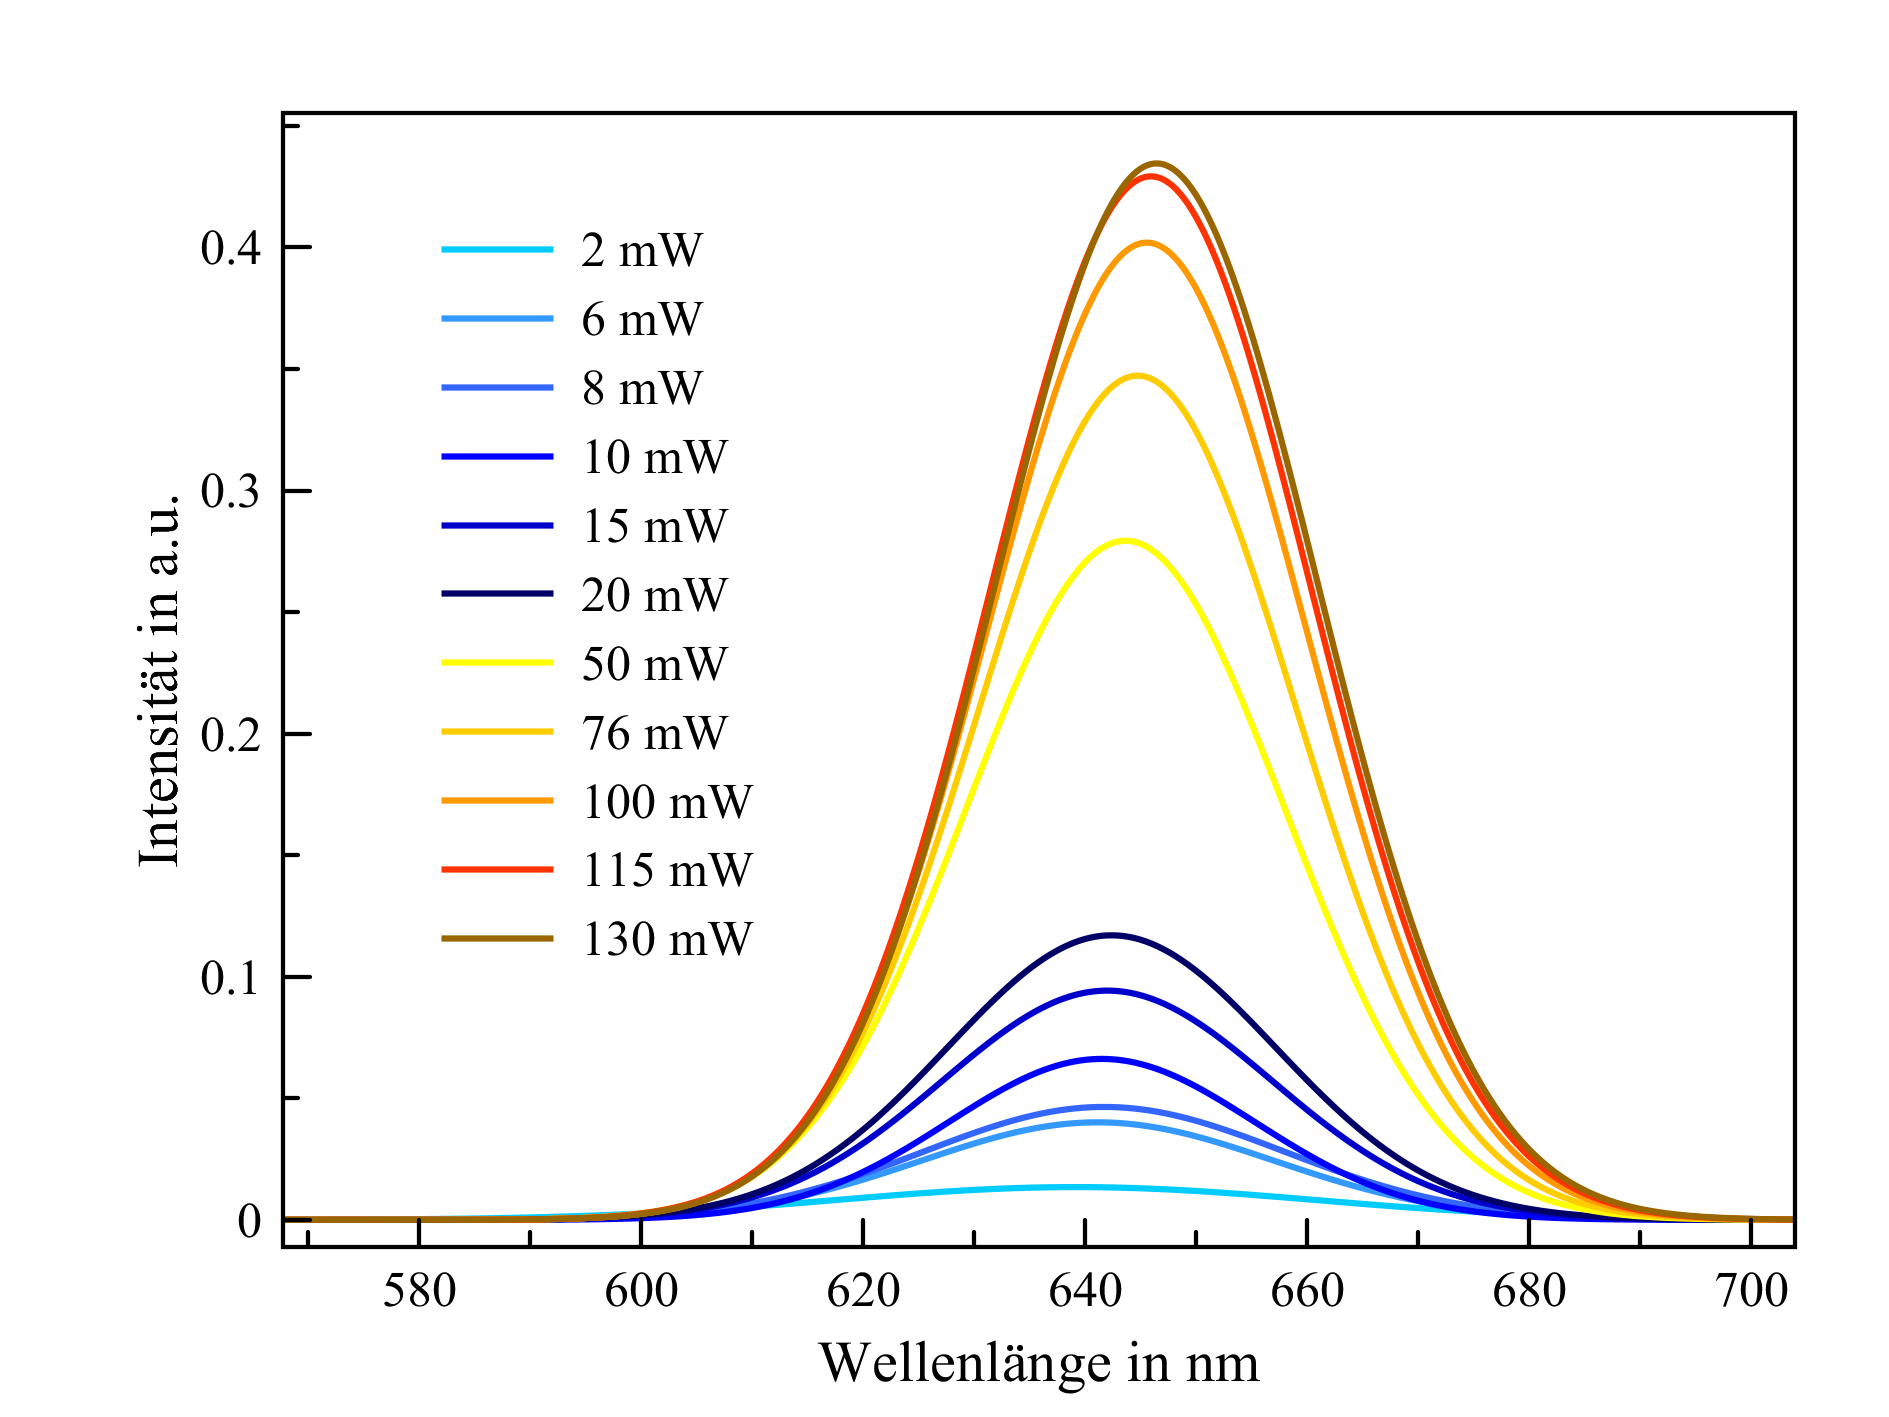
\includegraphics[width=\textwidth]{plots/Powerdependence_645nm.png}
  \end{subfigure}
  \begin{subfigure}{0.46\textwidth}
    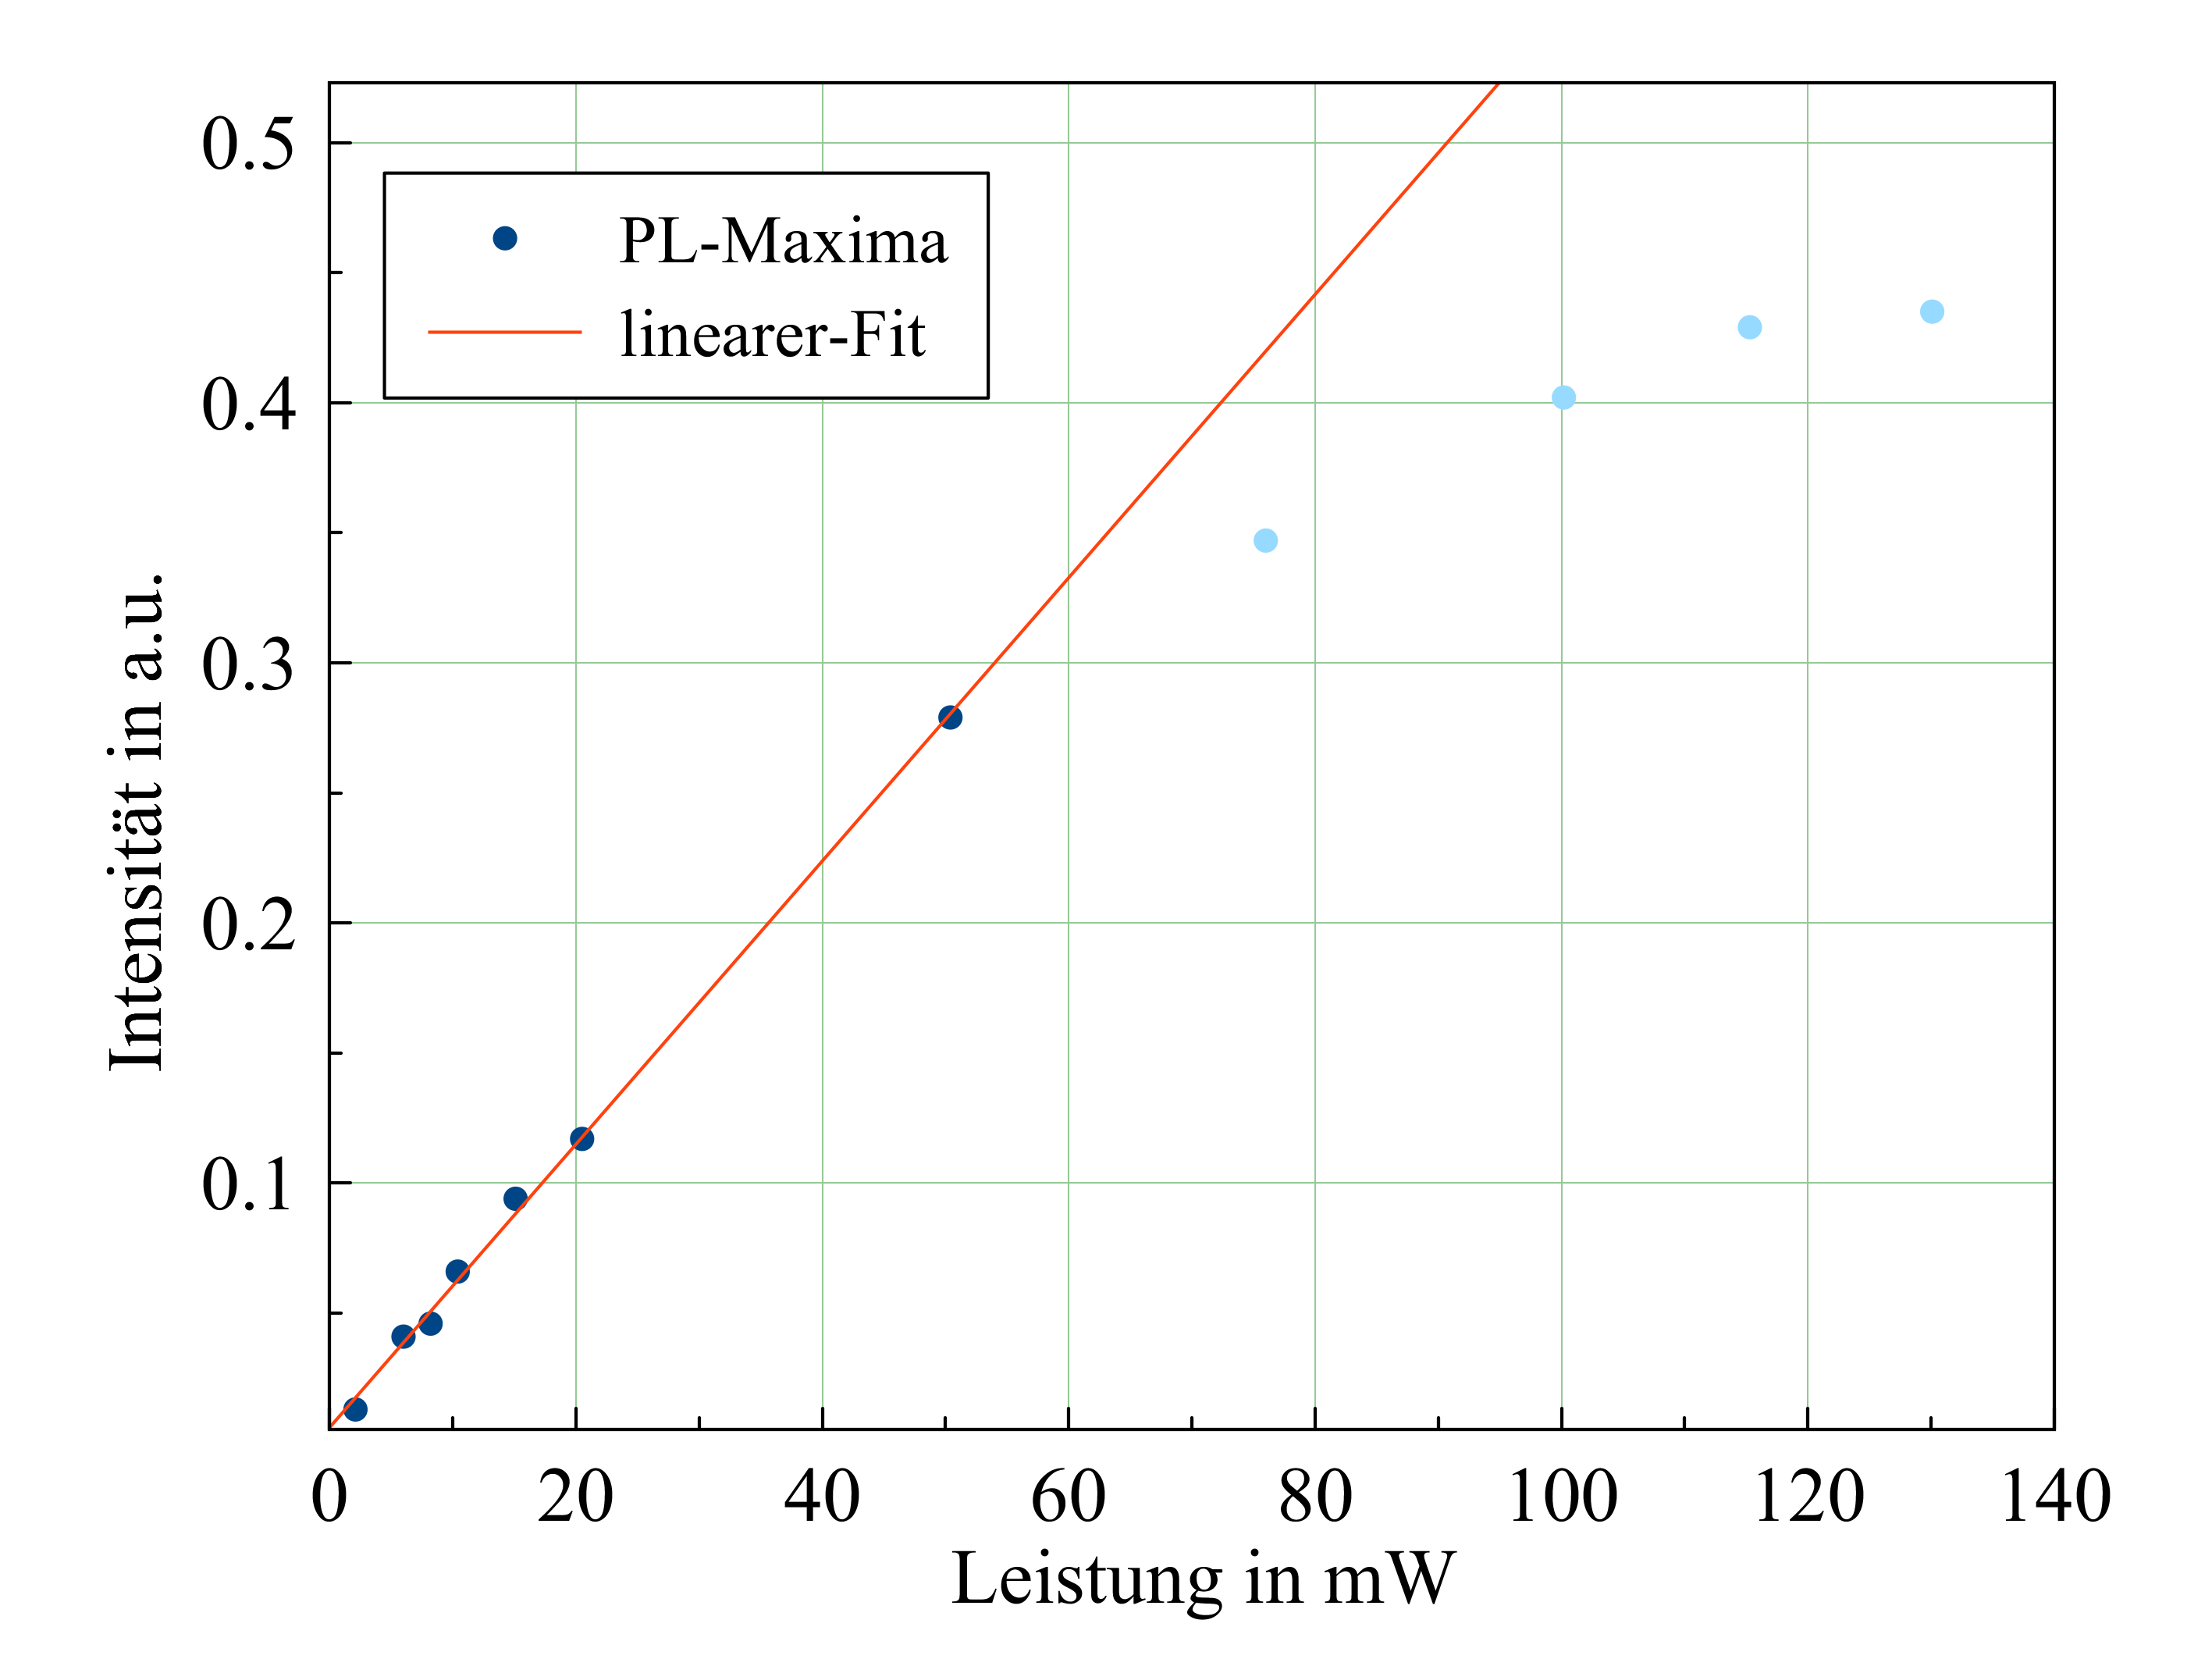
\includegraphics[width=\textwidth]{plots/Powerdepfit_645.png}
  \end{subfigure}
  \caption{Abhängigkeit der Photolumineszenz von der Eingangsleistung für eine Probe mit PL-Wellenlänge $\lambda_h = \SI{645}{\nano\meter}$. \textbf{Links:} Kurvenschar der Ausgleichsrechnungen der PL-Spektren für unterschiedliche Leistungen. \textbf{Rechts:} Darstellung der Maxima der Ausgleichskurven und Fit des linearen Anstiegs.}
  \label{fig:Podep645}
\end{figure}

Weiterhin sind Schwankungen der Position der maximalen Emissionsintensität der
Photolumineszenz auffällig. Die Position der maximalen Emissionsintensität ist für
beide Messungen in Abbildung \ref{fig:posem} aufgetragen. Es zeigt sich ein
klarer Anstieg der Emissionswellenlänge für die $\lambda_h=\SI{645}{\nano\meter}$
Probe. Aus den Ergebnissen der Messungen an der $\lambda_h=\SI{520}{\nano\meter}$
lassen sich keine klaren Abhängigkeiten ableiten.
\begin{figure}[H]
  \centering
  \begin{subfigure}{0.49\textwidth}
    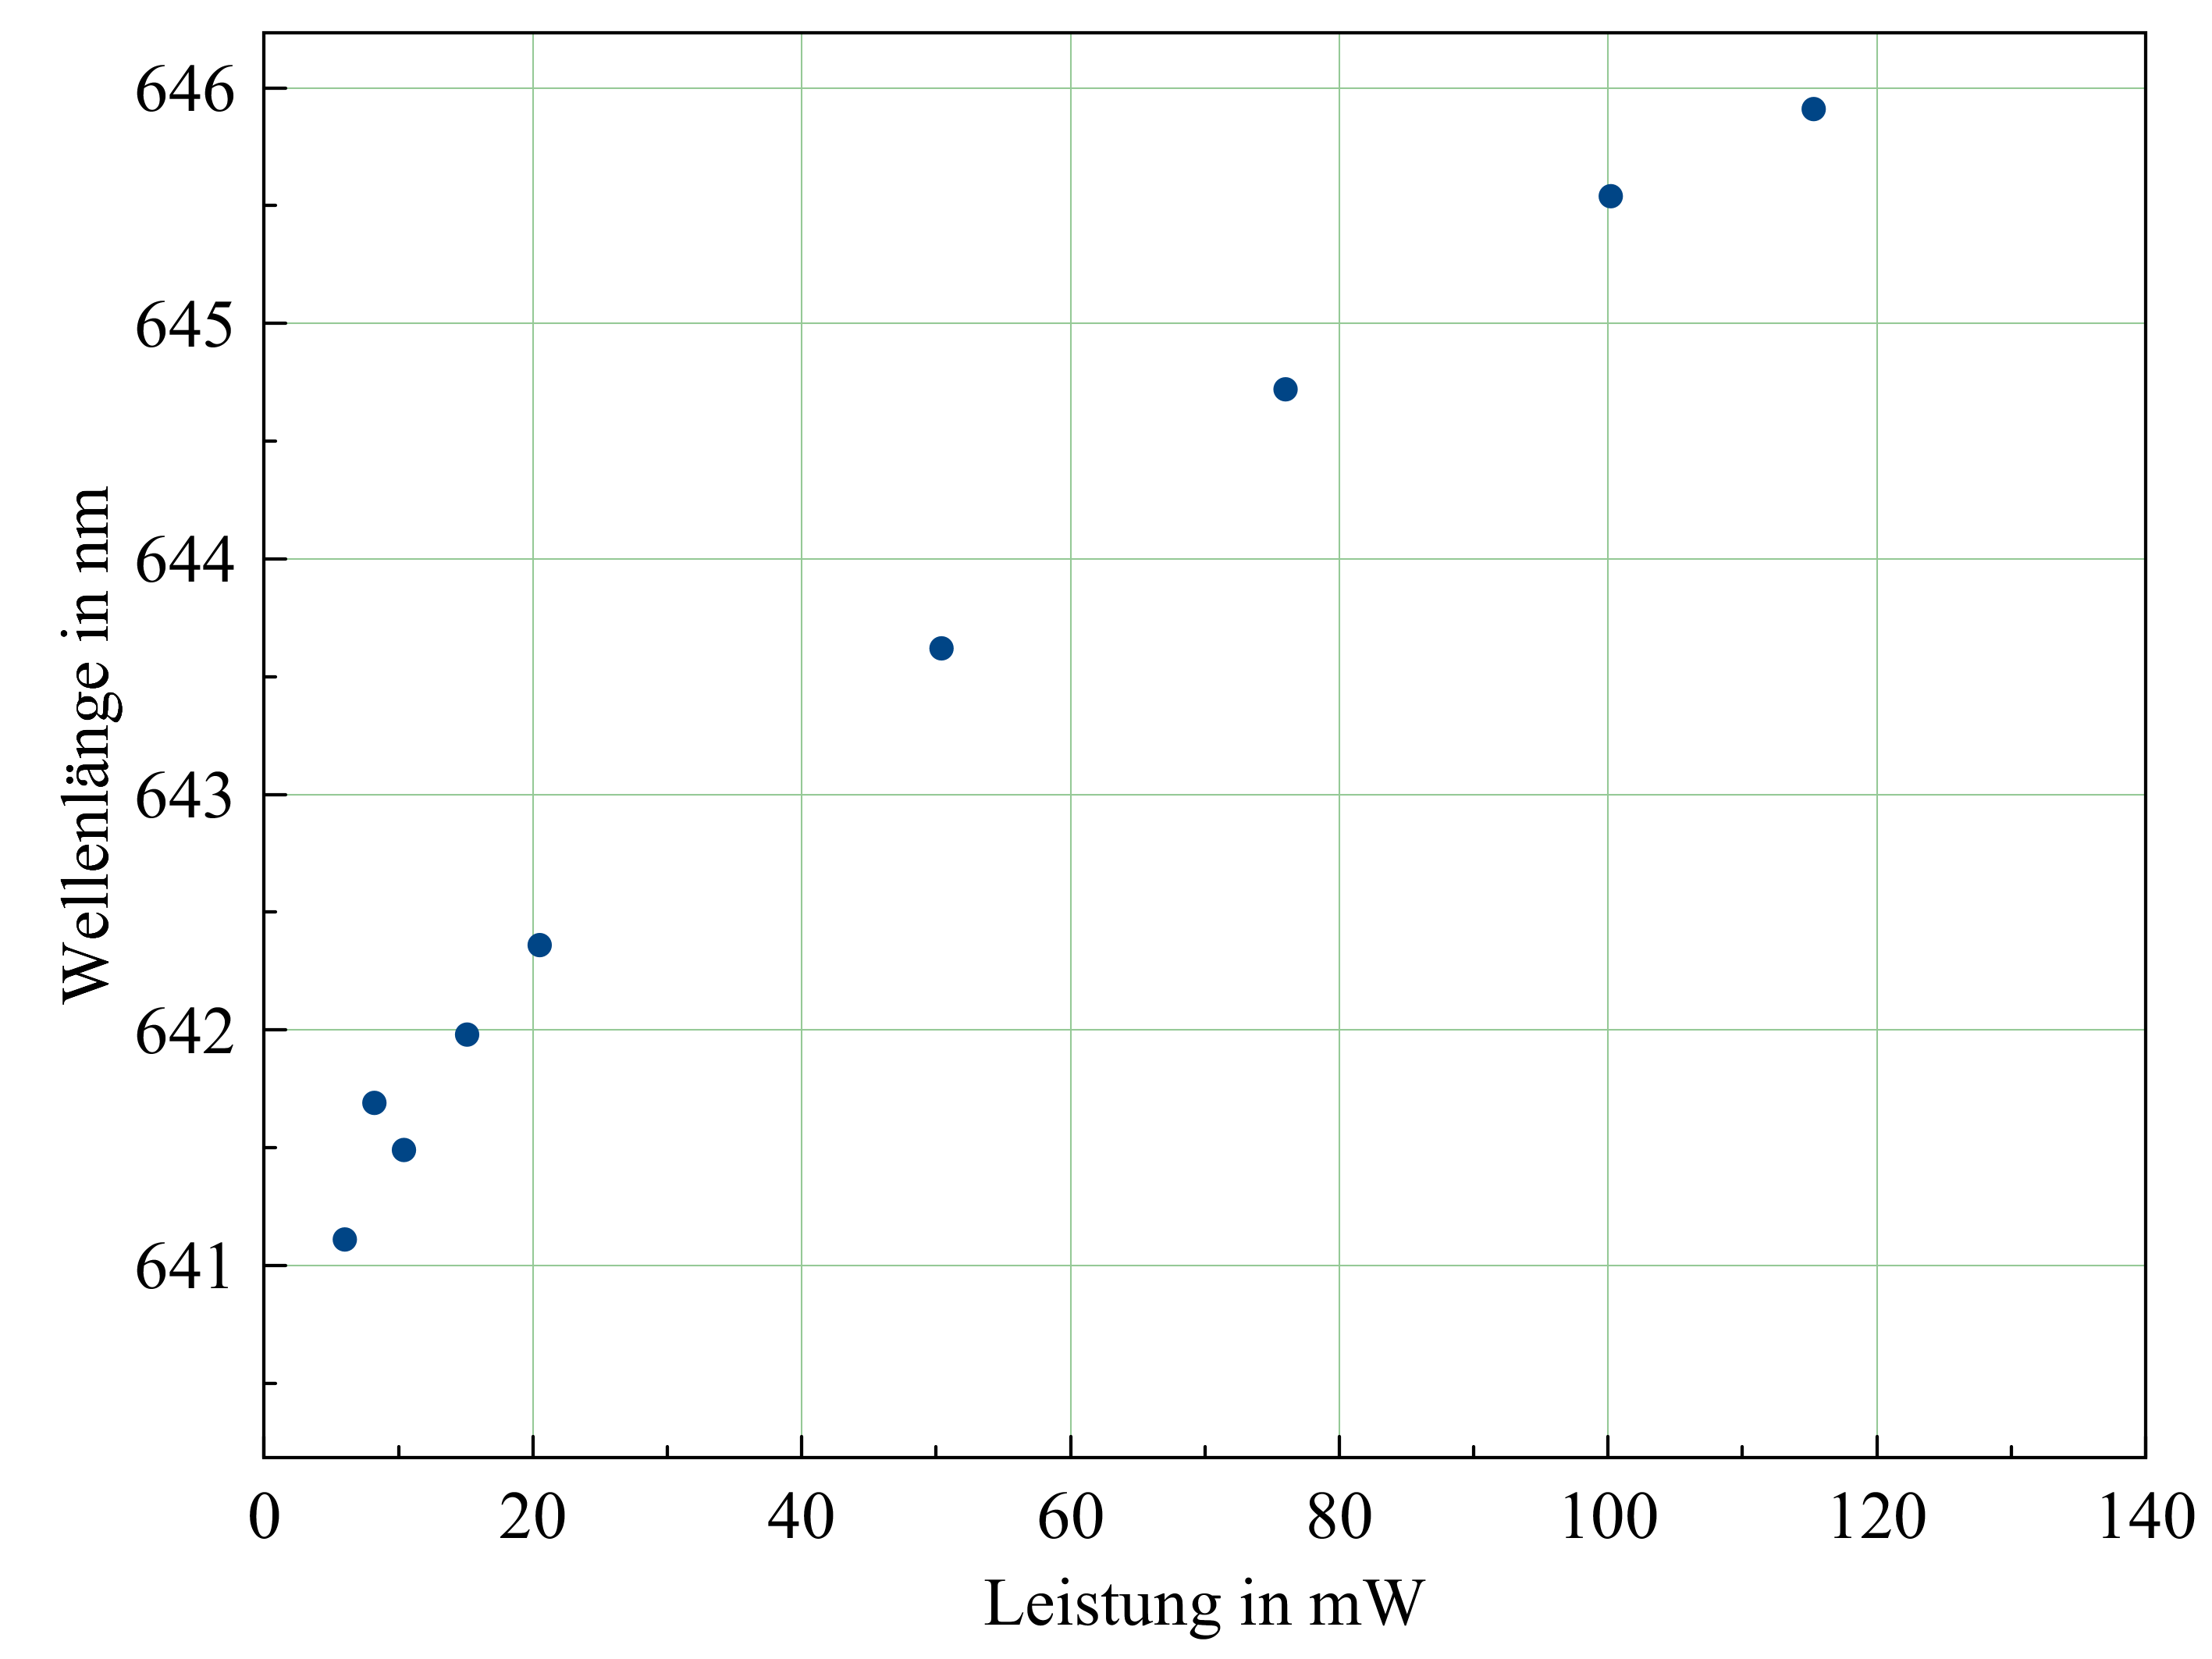
\includegraphics[width=\textwidth]{plots/posemplot_645nm.png}
    \caption{$\lambda_h = \SI{645}{\nano\meter}$}
  \end{subfigure}
  \begin{subfigure}{0.49\textwidth}
    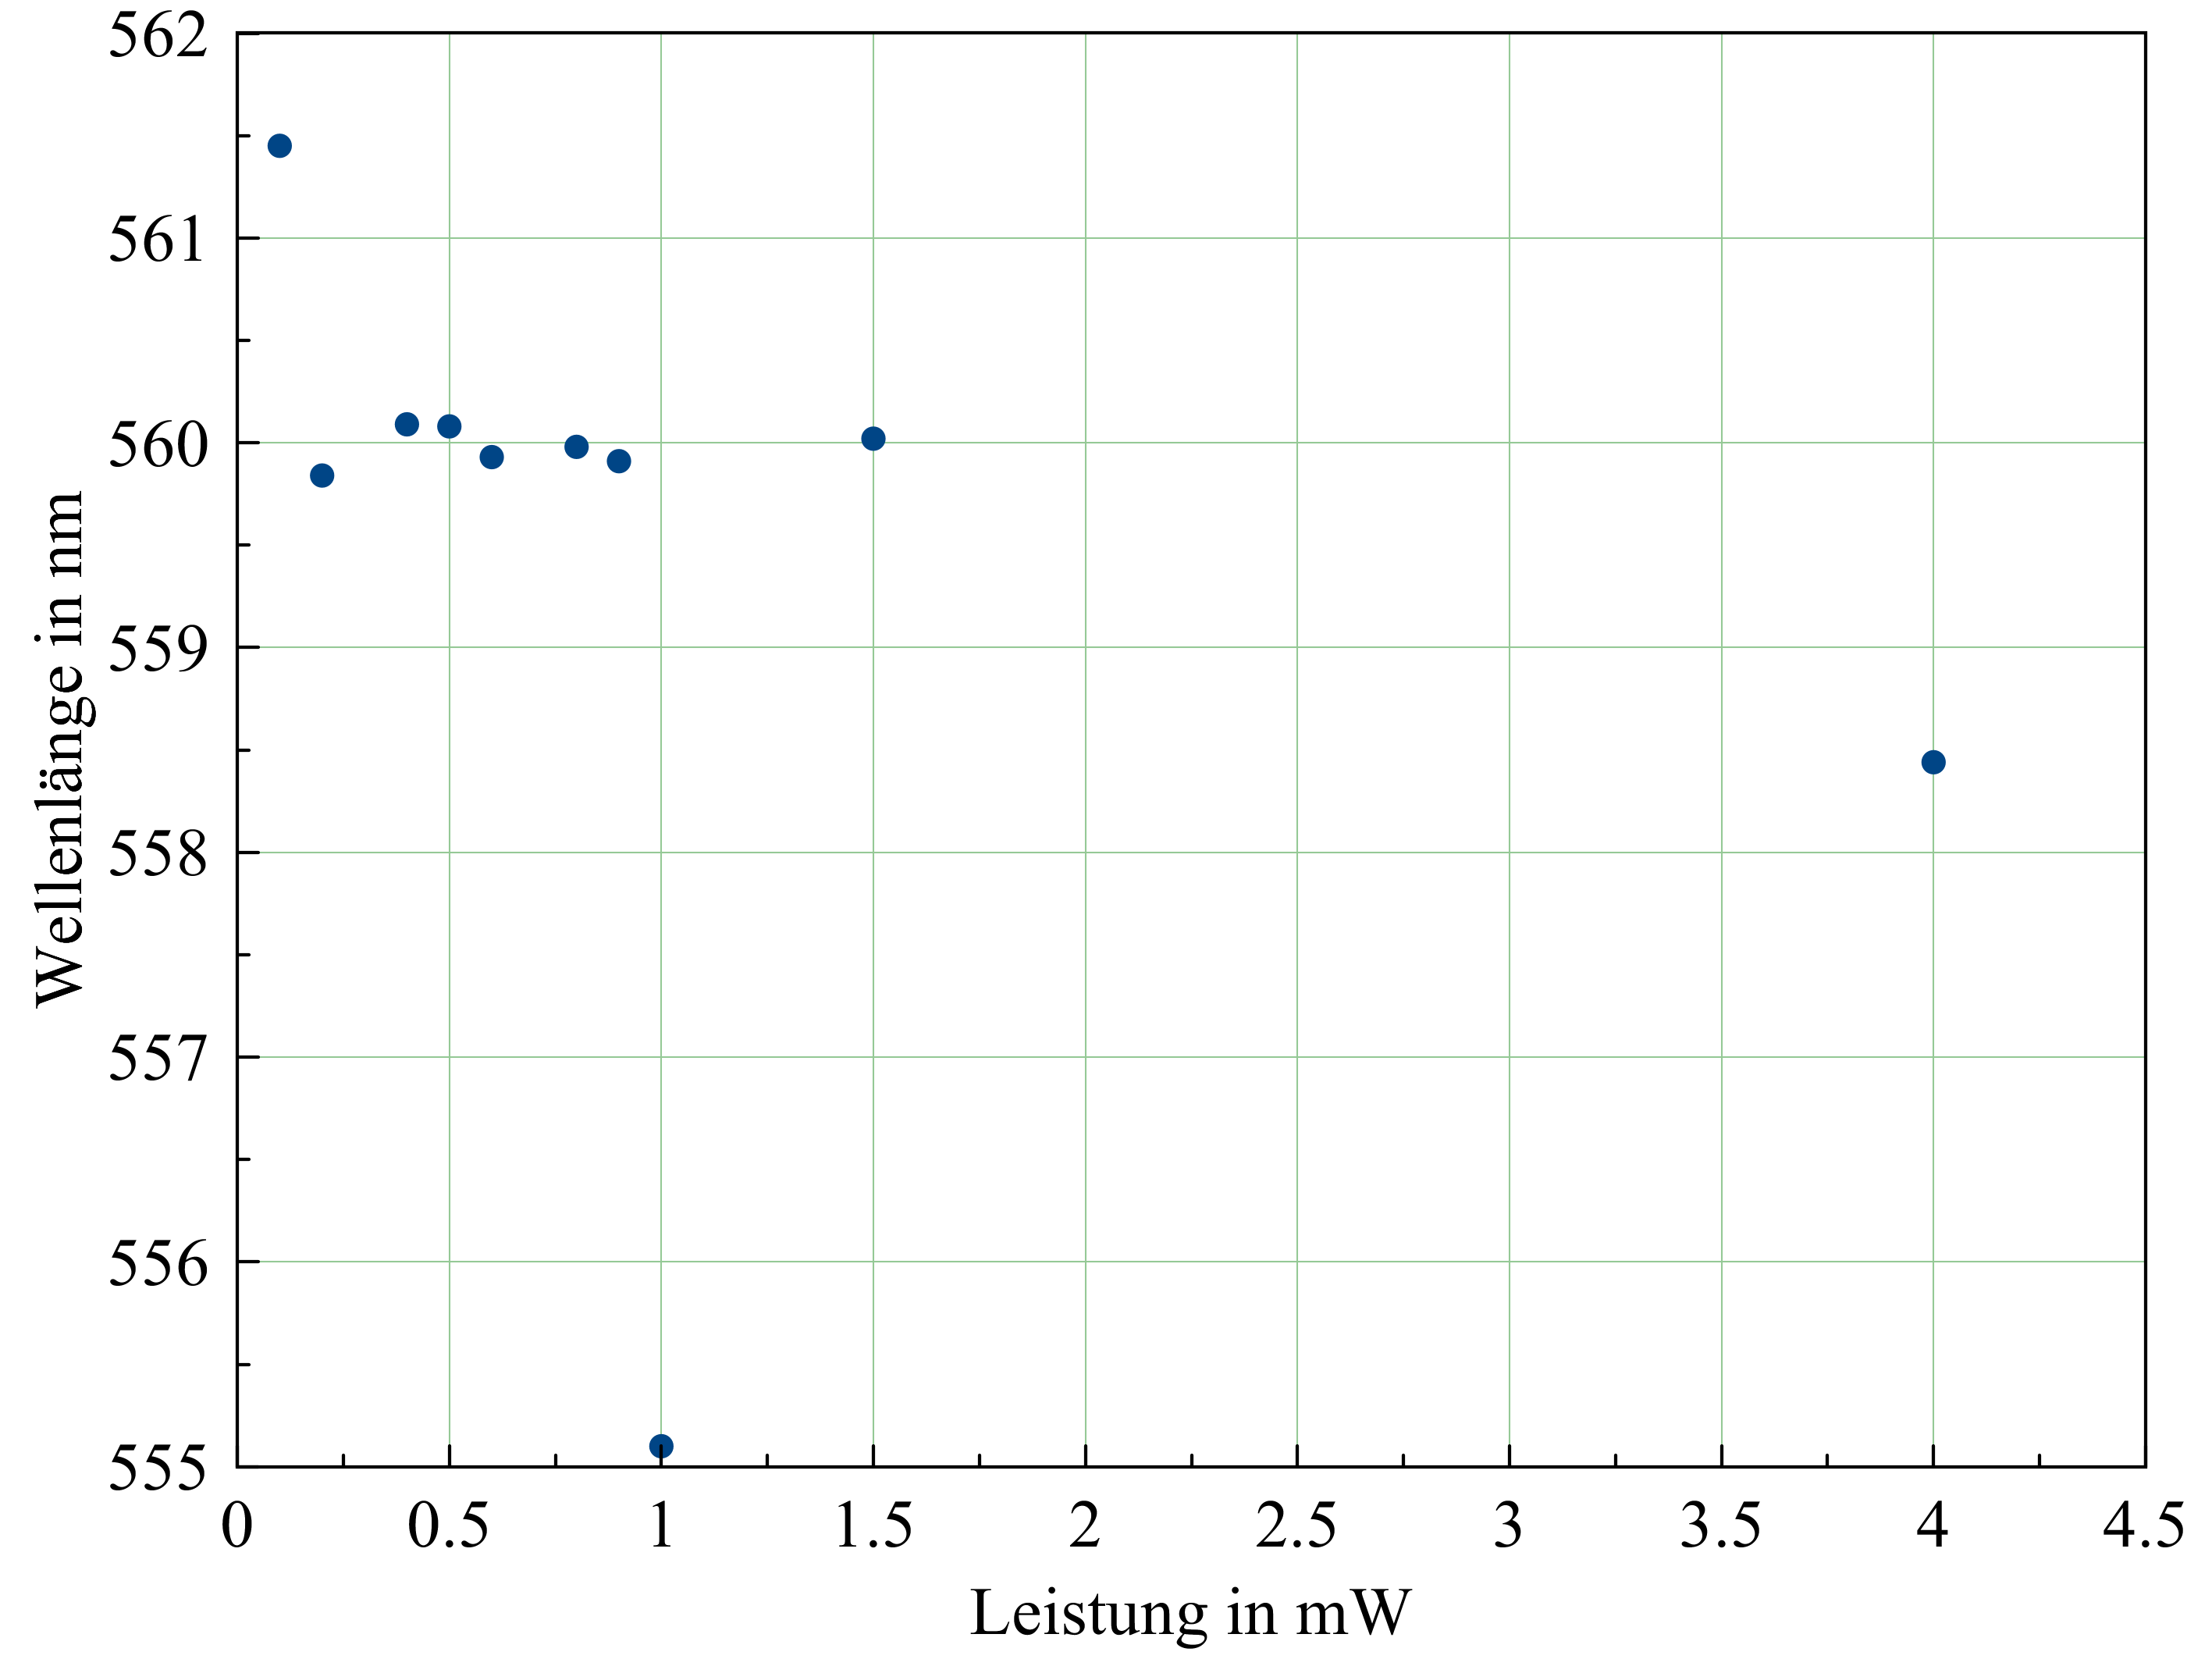
\includegraphics[width=\textwidth]{plots/posemplot_520.png}
    \caption{$\lambda_h = \SI{520}{\nano\meter}$}
  \end{subfigure}
  \caption{Abhängigkeit der Position des Emissionsmaximums von der Eingangsleistung.}
  \label{fig:posem}
\end{figure}

In den Abbildungen \ref{fig:Podep520} und ~\ref{fig:Podep645} ist außerdem ein
Änderung der Halbwertsbreiten der Emissionspeaks mit steigender Leistung
erkennbar. Der Zusammenhang von Eingangsleistung und Halbwertsbreite der Emissionspeaks
ist daher in Abbildung \ref{fig:FWHM} explizit dargestellt.

\begin{figure}[H]
  \centering
    \begin{subfigure}{0.49\textwidth}
      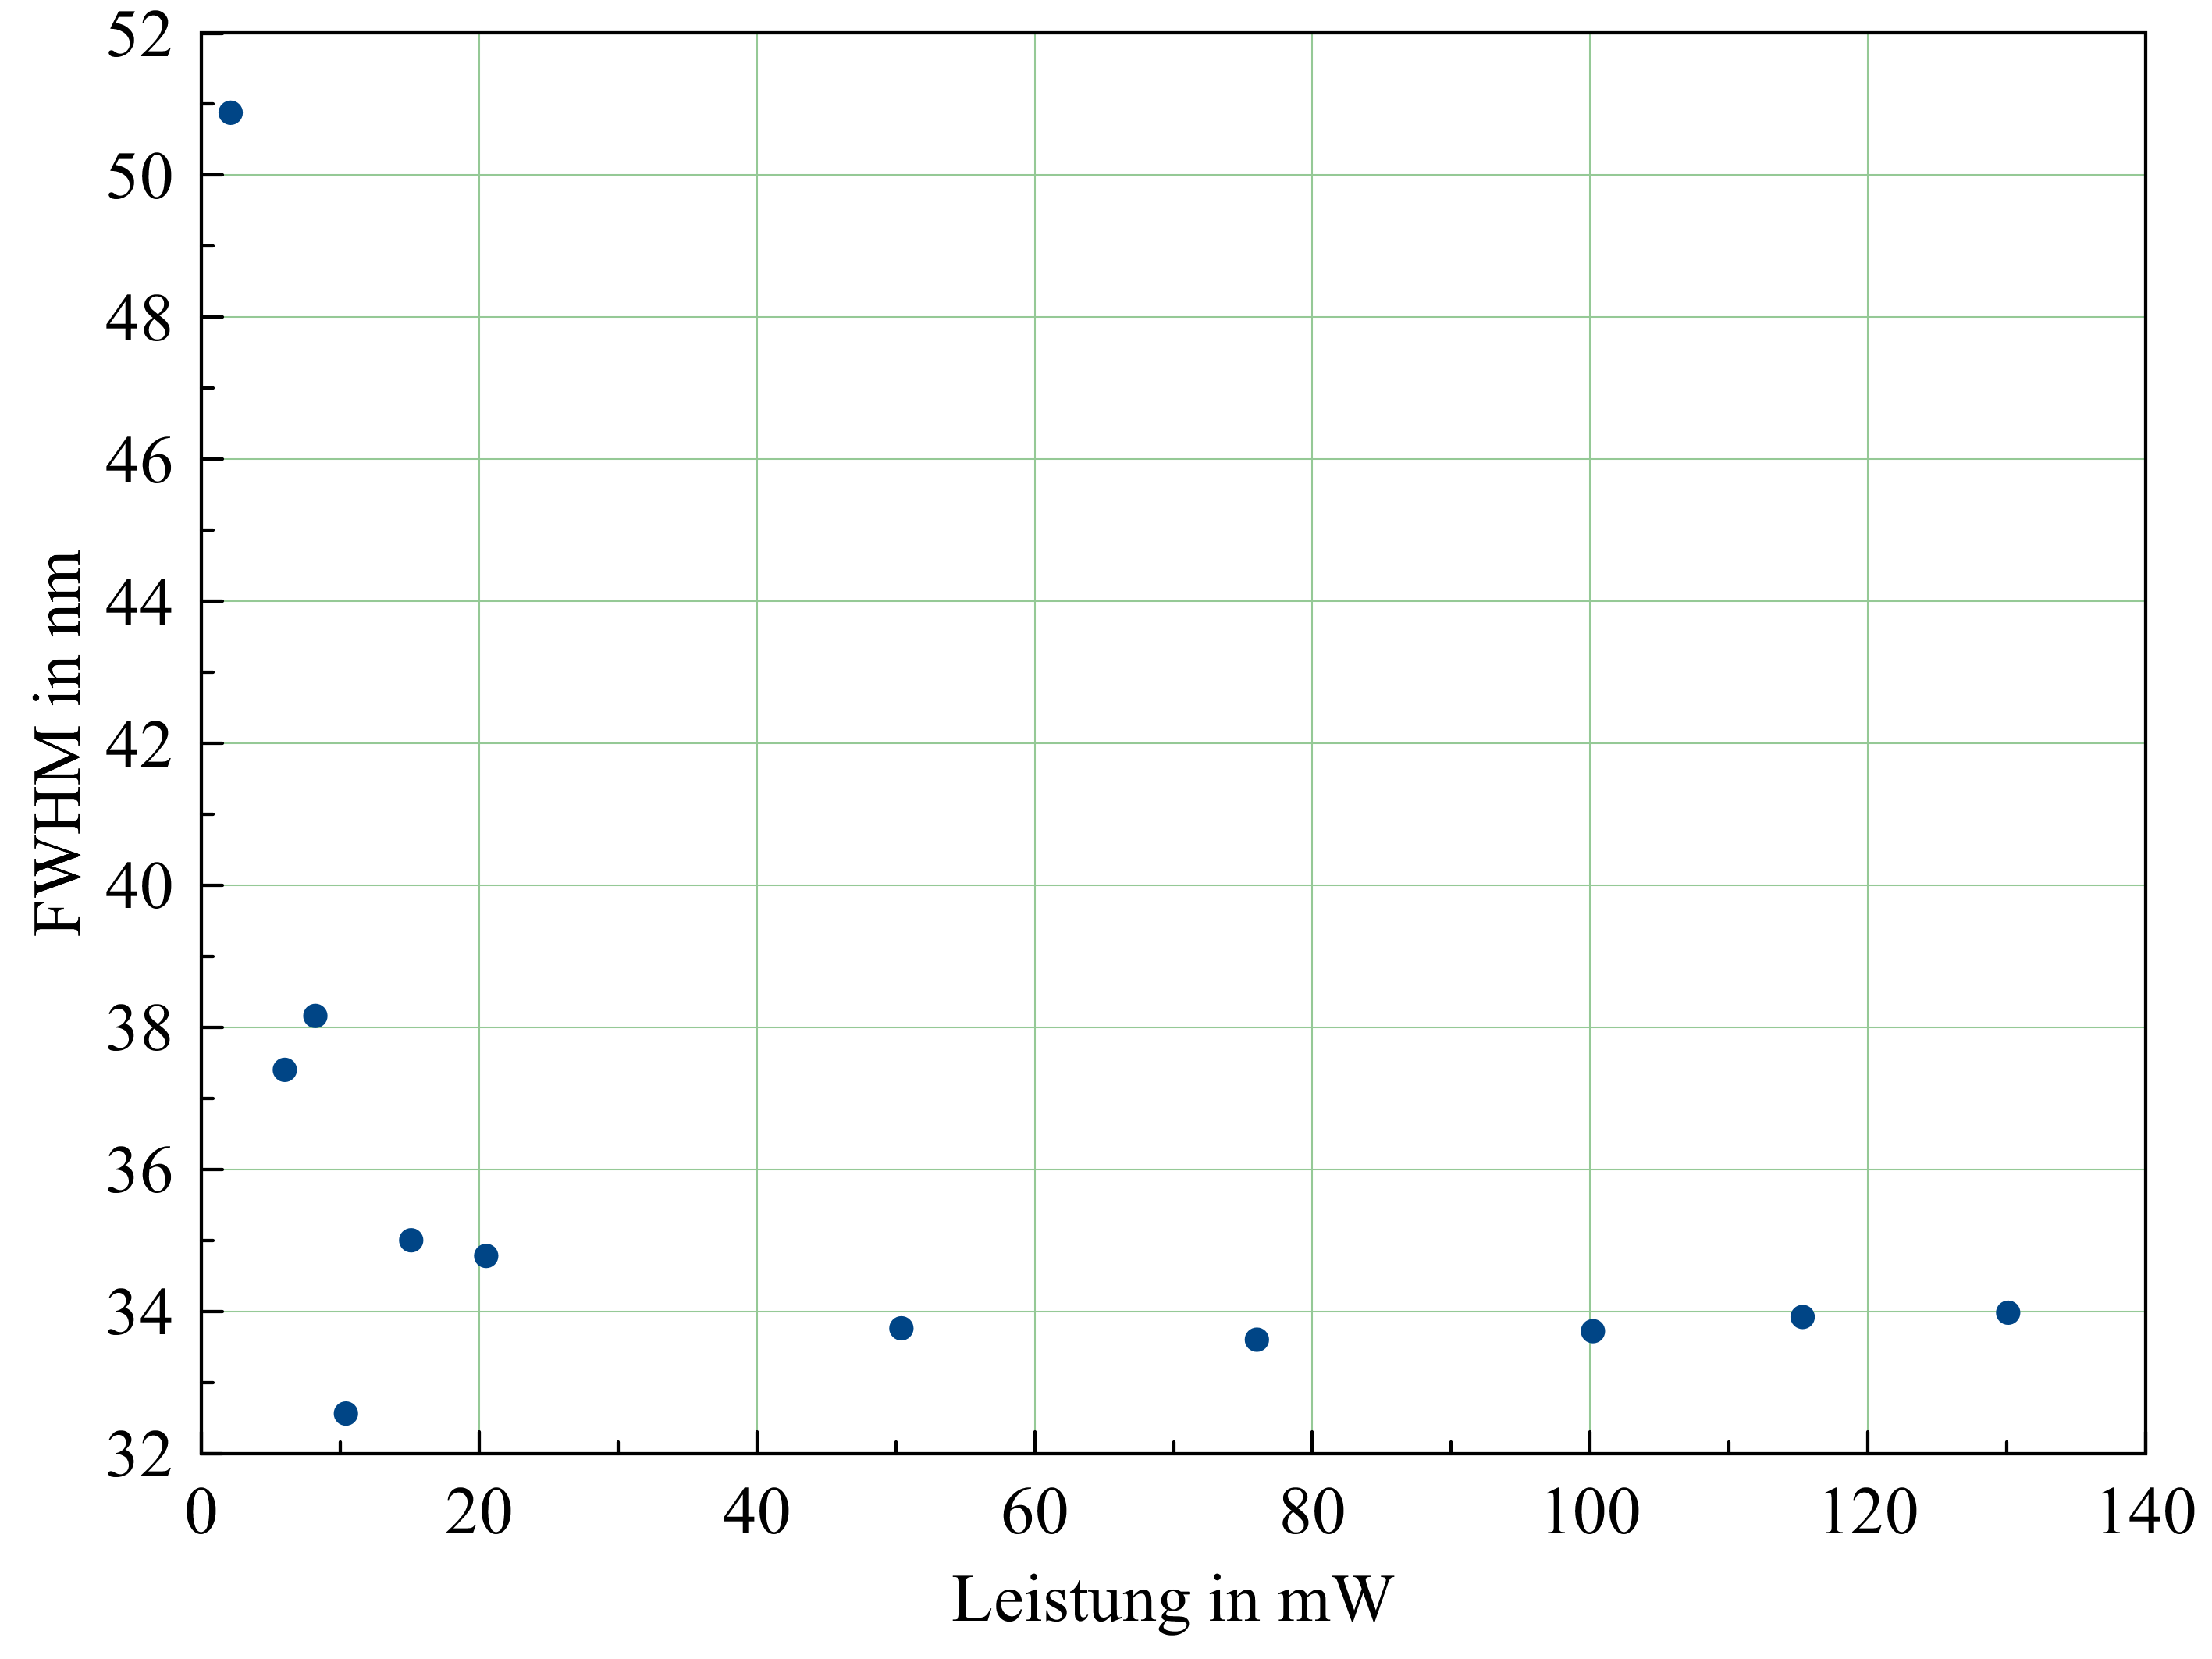
\includegraphics[width=\textwidth]{plots/FWHMplot_645.png}
      \caption{$\lambda_h = \SI{645}{\nano\meter}$}
    \end{subfigure}
    \begin{subfigure}{0.49\textwidth}
      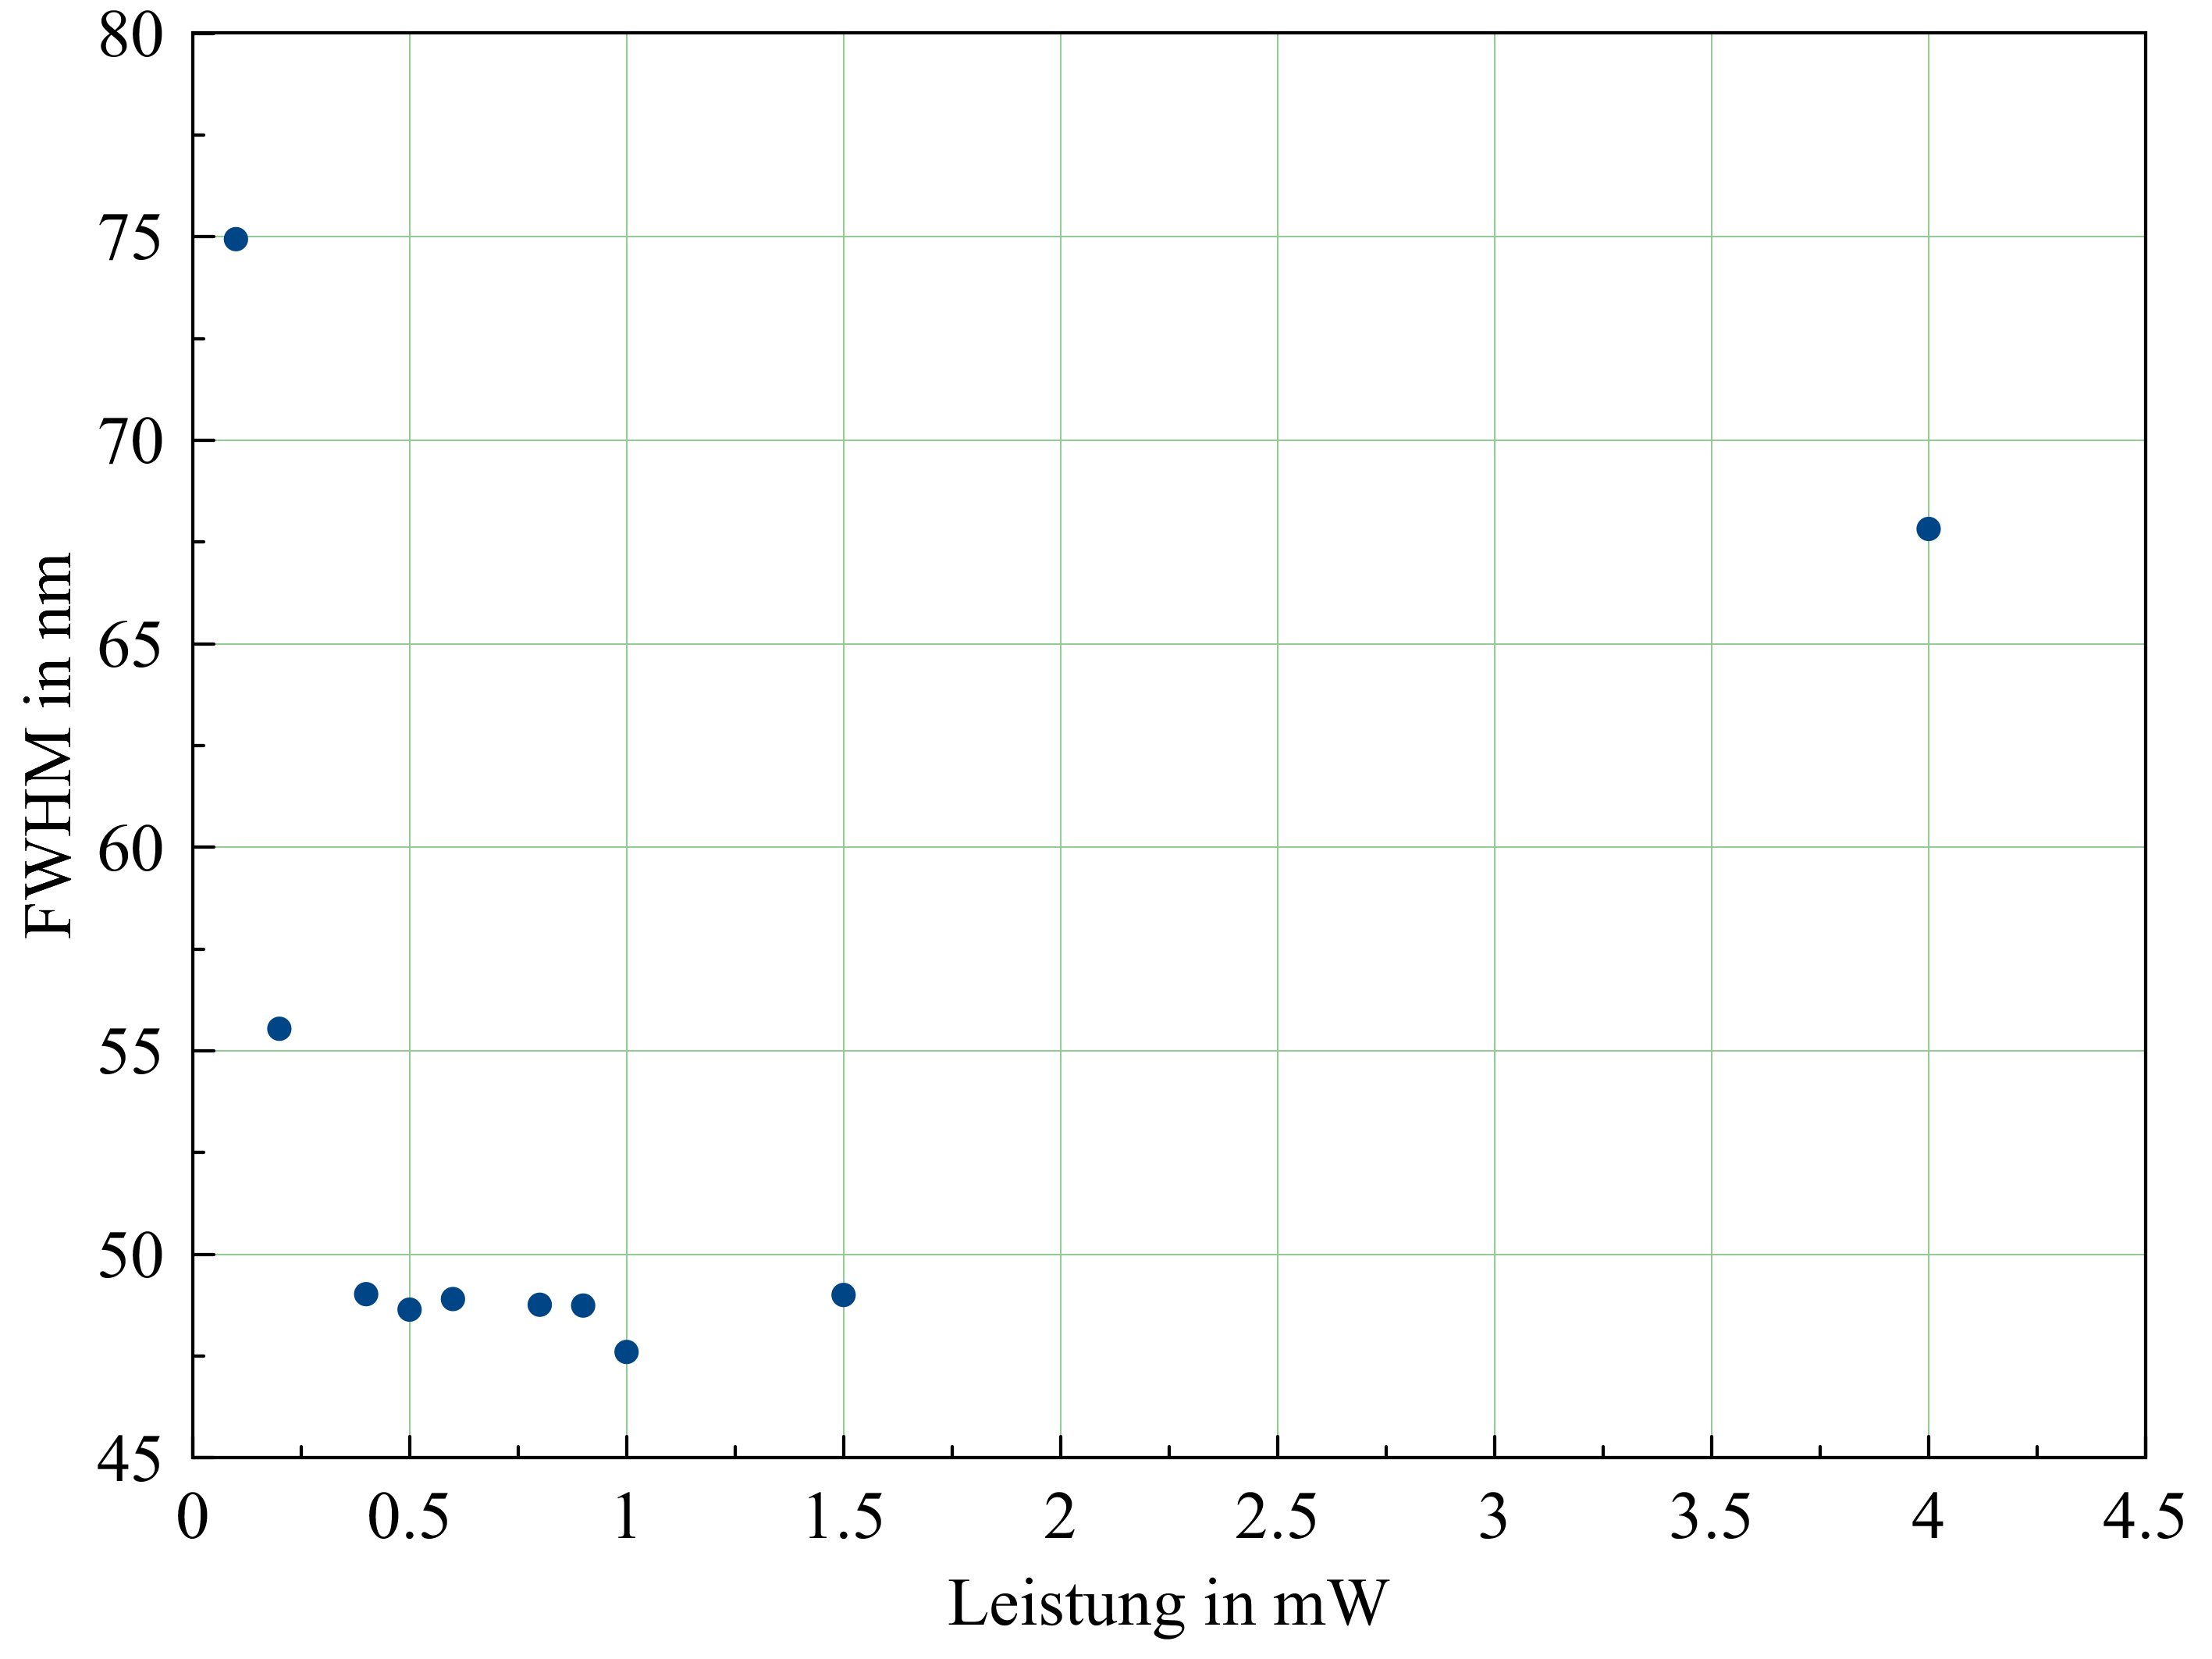
\includegraphics[width=\textwidth]{plots/FWHMplot_520.png}
      \caption{$\lambda_h = \SI{520}{\nano\meter}$}
    \end{subfigure}
  \caption{Abhängigkeit der Halbwertsbreiten (FWHM) von der Eingangsleistung.}
  \label{fig:FWHM}
\end{figure}
Für kleine Eingangsleistungen ergeben sich bei
der $\lambda_h=\SI{645}{\nano\meter}$ Probe
hohe Halbwertsbreiten, welche mit zunehmender Leistung
schnell kleiner werden und sich dann einem konstanten Wert annähern.
Die Halbwertsbreiten der $\lambda_h=\SI{520}{\nano\meter}$ Probe
zeigen, bis auf den bei $\SI{4}{\milli\watt}$ aufgenommenen Messwert, ein ähnliches Verhalten.

\subsection{Abhängigkeit der PL von der Polarisation}
\label{sec:Polarisation}
Um eine Abhängigkeit von der Polarisation des eingestrahlten Lichtes festzustellen,
wurden für drei verschiedene lineare Polarisationen Photolumineszenzspektren einer
Probe aufgenommen. Anregungswellenlänge und  Eingangsleistung wurden hier nicht verändert.
Aus den gemessenen Spektren (Abbildung \ref{fig:Polarisation}) geht hervor, dass die
Photolumineszenz nicht von der Polarisation des anregenden Lichtes abhängt.
\begin{figure}[H]
  \centering
  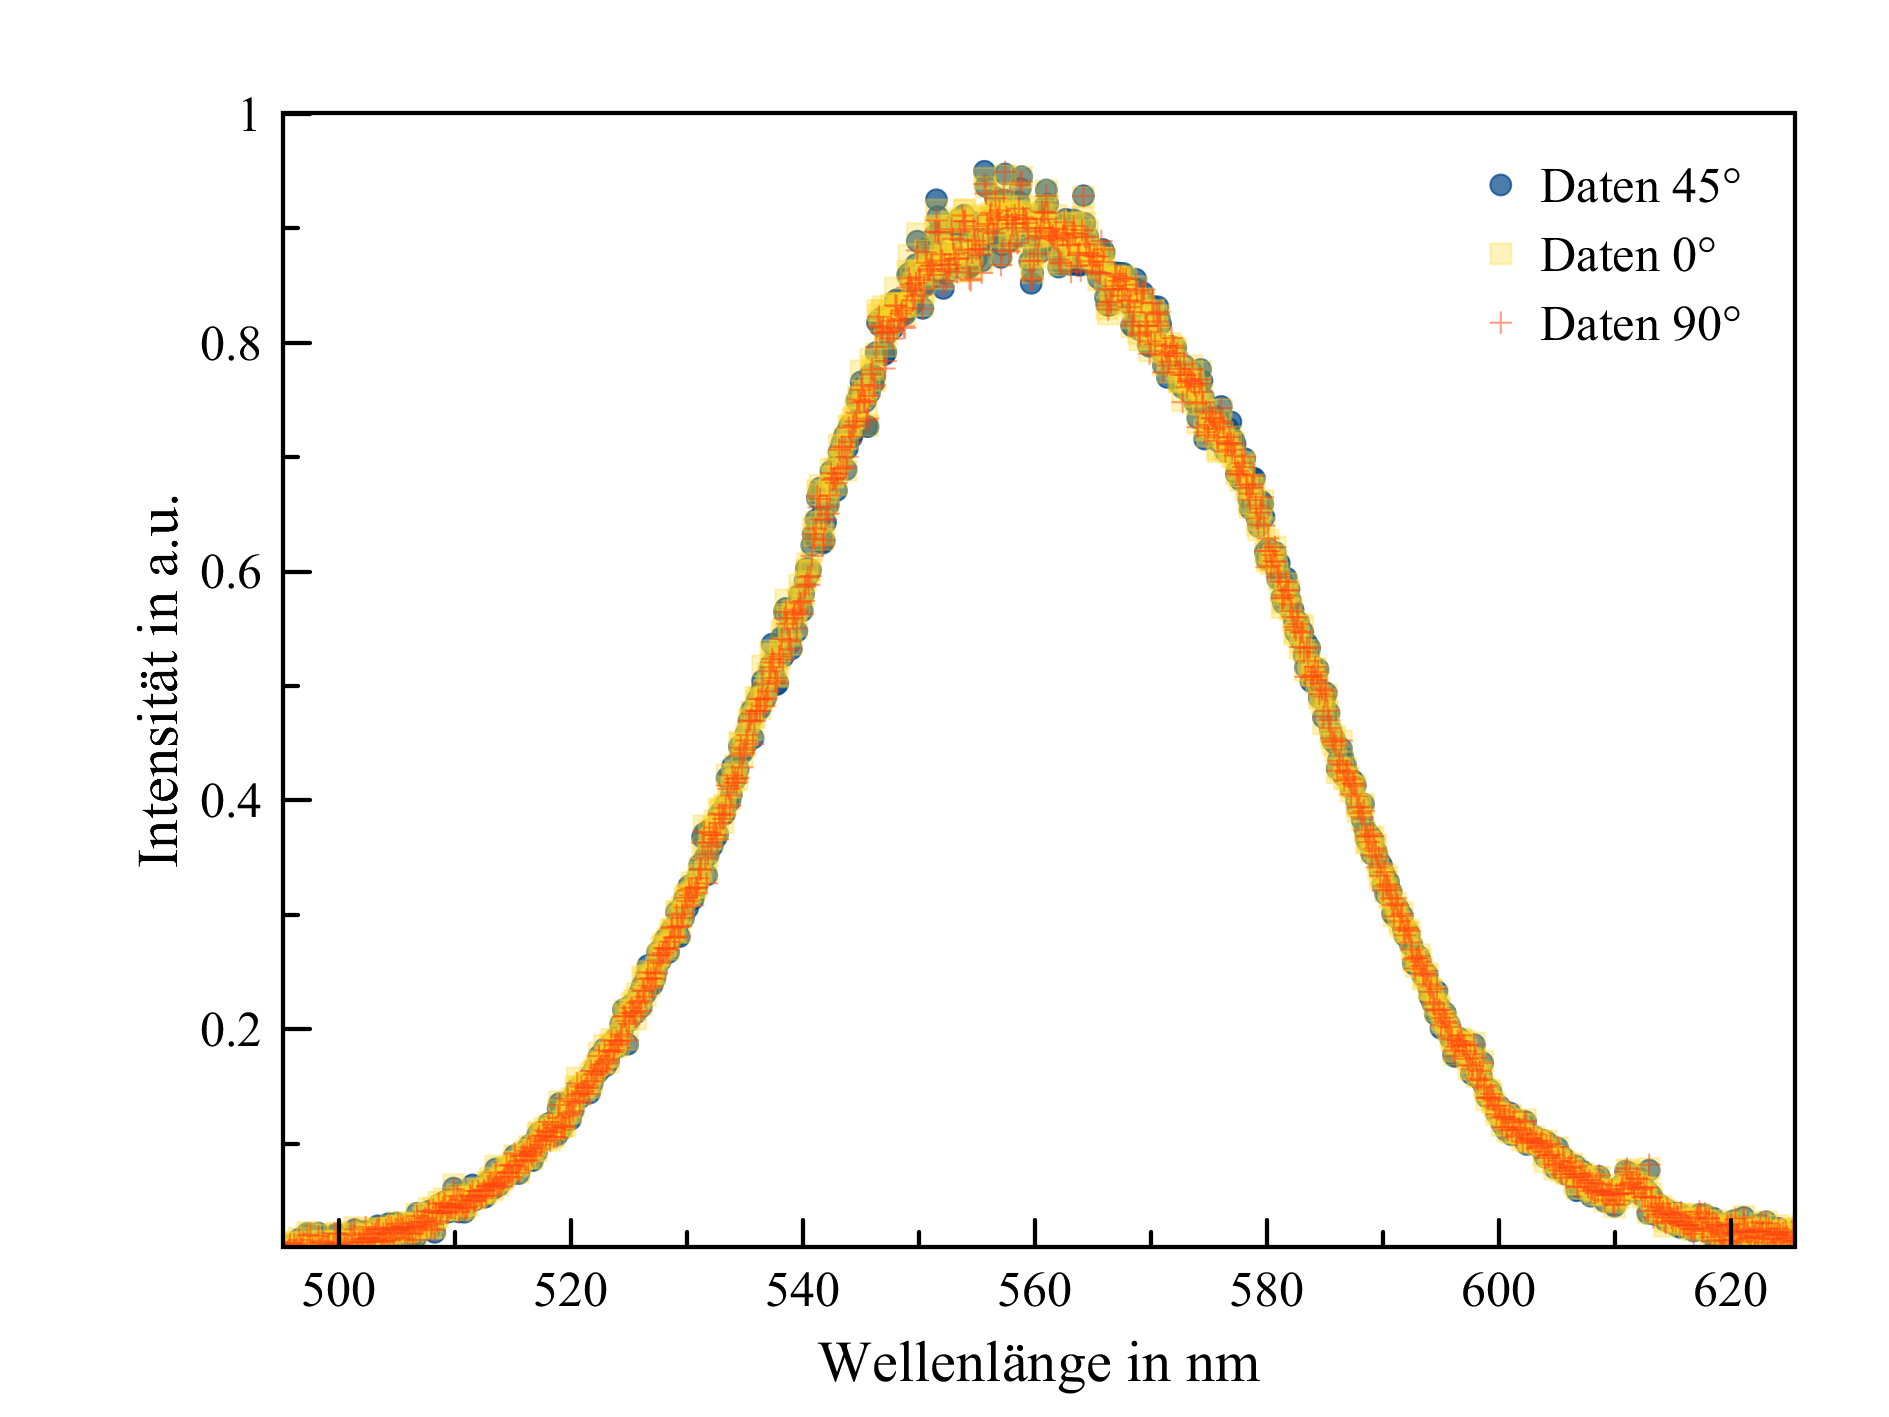
\includegraphics[width=0.7\textwidth]{plots/Poldepplot.png}
  \caption{Abhängigkeit der Photolumineszenz der $\lambda_h=\SI{520}{\nano\meter}$
   Probe bei einer Anregungswellenlänge von $\lambda=\SI{405}{\nano\meter}$ und einer Eingangsleistung von $\SI{1,5}{\milli\watt}$.}
   \label{fig:Polarisation}
\end{figure}

\subsection{Photolumineszenz bei anderen Anregungsenergien}
\label{subsec:34}
Zuletzt wurden Photolumineszentspektren aller drei Proben für zwei weitere
Anregungswellenlängen, $\SI{520}{\nano\meter}$ und $\SI{470}{nm}$ aufgenommen.
Die Ergebnisse sind in den Abbildungen \ref{fig:PL_645} bis \ref{fig:PL_520} dargestellt.
In Abbildung \ref{fig:PL_645_470} ist die Sättigung des CCD-Chips deutlich zu sehen.
Für die $\lambda_h=\SI{645}{\nano\meter}$ ist keine Photolumineszenz der
Probe auszumachen und es ist nur die Reflexion des Anregungslichts zu sehen. Daher wurden für diese Messung keine weiteren Ausgleichsrechnung neben der Ermittlung der Breite und Position des Reflexionspeaks der Anregung durchgeführt. Der fettgedruckte Wert in Tabelle \ref{tab:weisslicht1} ist der über den Filter eingestellte Wert des Anregungslichts und dient nur als Referenz.
In den weiteren Spektren ist diese Reflexion klar von dem,
durch die Photolumineszenz entstehenden Peak, unterscheidbar.
Die Halbwertsbreiten des Anregungslichts $\Gamma_{\text{ex}}$ und der Emission $\Gamma_{\text{em}}$, sowie die Position der Anregungs- und Emissionspeaks $\lambda_{\text{ex}}$ und $\lambda_{\text{em}}$, sind in den Tabellen \ref{tab:weisslicht1} bis \ref{tab:weisslicht3} zusammengestellt.

\begin{table}[H]
  \centering
  \caption{Halbwertsbreiten $\Gamma$ und Peakposition $\lambda$ der Photolumineszenzpeaks der $\lambda_h = \SI{645}{\nano\meter}$ Probe für zwei weitere Wellenlängen. Der Index "ex" steht dabei für das anregende Licht und der Index "em" für die emittierte Photolumineszenz.}
  \label{tab:weisslicht1}
\begin{tabular}{c|c|c|c}
  \toprule
     $\lambda_{\text{ex}}$ in $\si{\nano\meter}$ & $\Gamma_{\text{ex}}$ in $\si{\nano\meter}$ & $\lambda_{\text{em}}$ in $\si{\nano\meter}$ & $\Gamma_{\text{em}}$ in $\si{\nano\meter}$ \\
     \midrule
     $520.031 \pm 0.009$ & $7.81 \pm 0.01$ &   &  \\
     \textbf{570} &                &     &    \\
  \bottomrule
\end{tabular}
\end{table}

\begin{table}[H]
  \centering
  \caption{Halbwertsbreiten $\Gamma$ und Peakposition $\lambda$ der Photolumineszenzpeaks der $\lambda_h = \SI{580}{\nano\meter}$ Probe für zwei weitere Wellenlängen. Der Index "ex" steht dabei für das anregende Licht und der Index "em" für die emittierte Photolumineszenz.}
  \label{tab:weisslicht2}
\begin{tabular}{c|c|c|c}
  \toprule
     $\lambda_{\text{ex}}$ in $\si{\nano\meter}$ & $\Gamma_{\text{ex}}$ in $\si{\nano\meter}$ & $\lambda_{\text{em}}$ in $\si{\nano\meter}$ & $\Gamma_{\text{em}}$ in $\si{\nano\meter}$ \\
  \midrule
  $520.00 \pm 0.02$ & $7.89 \pm 0.02 $ & $594.1 \pm 0.7 $ & $35.3 \pm 0.7$ \\
  $469.01 \pm 0.04$ & $8.34 \pm 0.05 $ & $593.0 \pm 0.1 $ & $36.2 \pm 0.2$ \\
   \bottomrule
\end{tabular}
\end{table}

\begin{table}[H]
  \centering
  \caption{Halbwertsbreiten $\Gamma$ und Peakposition $\lambda$ der Photolumineszenzpeaks der $\lambda_h = \SI{520}{\nano\meter}$ Probe für zwei weitere Wellenlängen. Der Index "ex" steht dabei für das anregende Licht und der Index "em" für die emittierte Photolumineszenz.}
  \label{tab:weisslicht3}
\begin{tabular}{c|c|c|c}
  \toprule
     $\lambda_{\text{ex}}$ in $\si{\nano\meter}$ & $\Gamma_{\text{ex}}$ in $\si{\nano\meter}$ & $\lambda_{\text{em}}$ in $\si{\nano\meter}$ & $\Gamma_{\text{em}}$ in $\si{\nano\meter}$ \\
     \midrule
     $520.17 \pm 0.02$ & $8.22 \pm 0.22 $ & $557.67 \pm 0.19 $ & $52.66 \pm 0.26$ \\
     $469.10 \pm 0.02 $ & $ 8.24 \pm 0.03 $ & $ 559.28 \pm 0.20 $ & $46.86 \pm 0.23$ \\
  \bottomrule
\end{tabular}
\end{table}
Es fällt auf, dass die Photolumineszenz eine deutlich höhere spektrale Breite aufweist, als die spektrale Breite der jeweiligen Anregung. Die Emissionswellenlängen $\lambda_{\text{em}}$ der einzelnen Proben weisen bei Anregung durch andere Wellenlängen nur sehr geringe Abweichungen voneinander auf. Allerdings ist auch hier eine Abweichung der Emissionswellenlänge der $\lambda_h = \SI{520}{\nano\meter}$ von der Herstellerangabe auffällig.
\begin{figure}[H]
  \centering
  \begin{subfigure}{0.49\textwidth}
    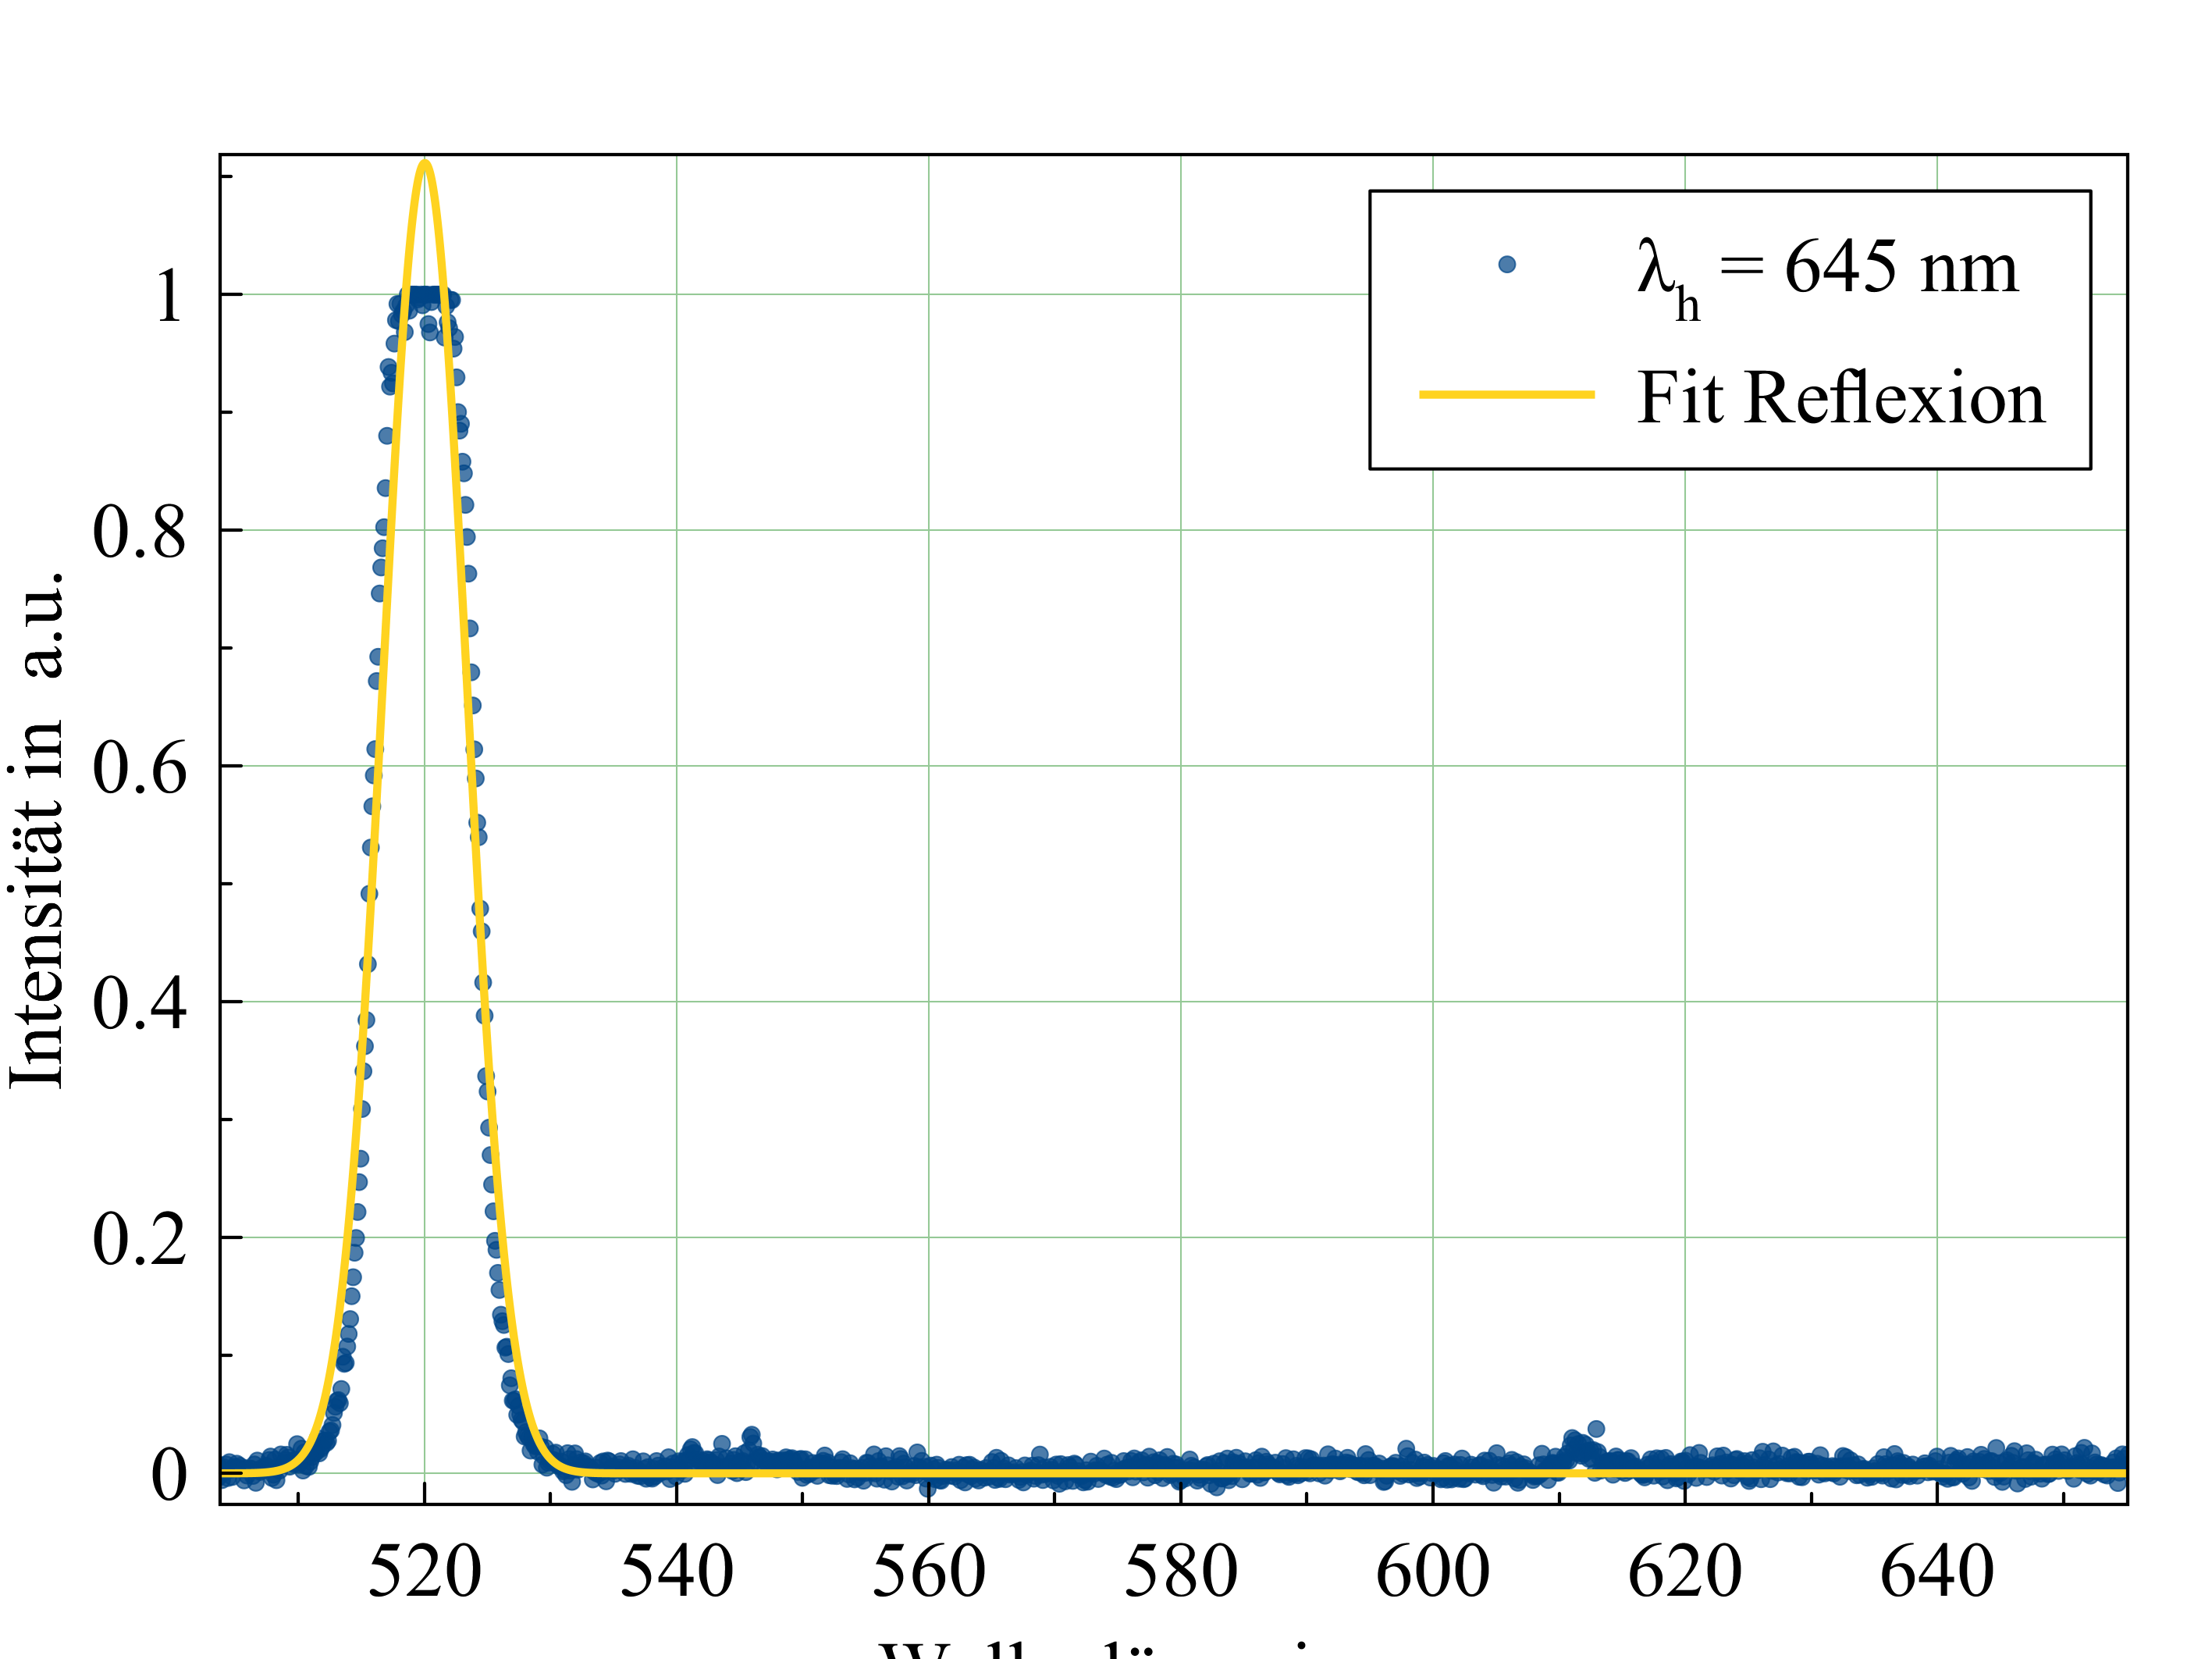
\includegraphics[width=\textwidth]{plots/Weisslicht_645_520.png}
    \caption{$\lambda=\SI{520}{\nano\meter}$}
    \label{fig:645_520}
  \end{subfigure}
  \begin{subfigure}{0.49\textwidth}
    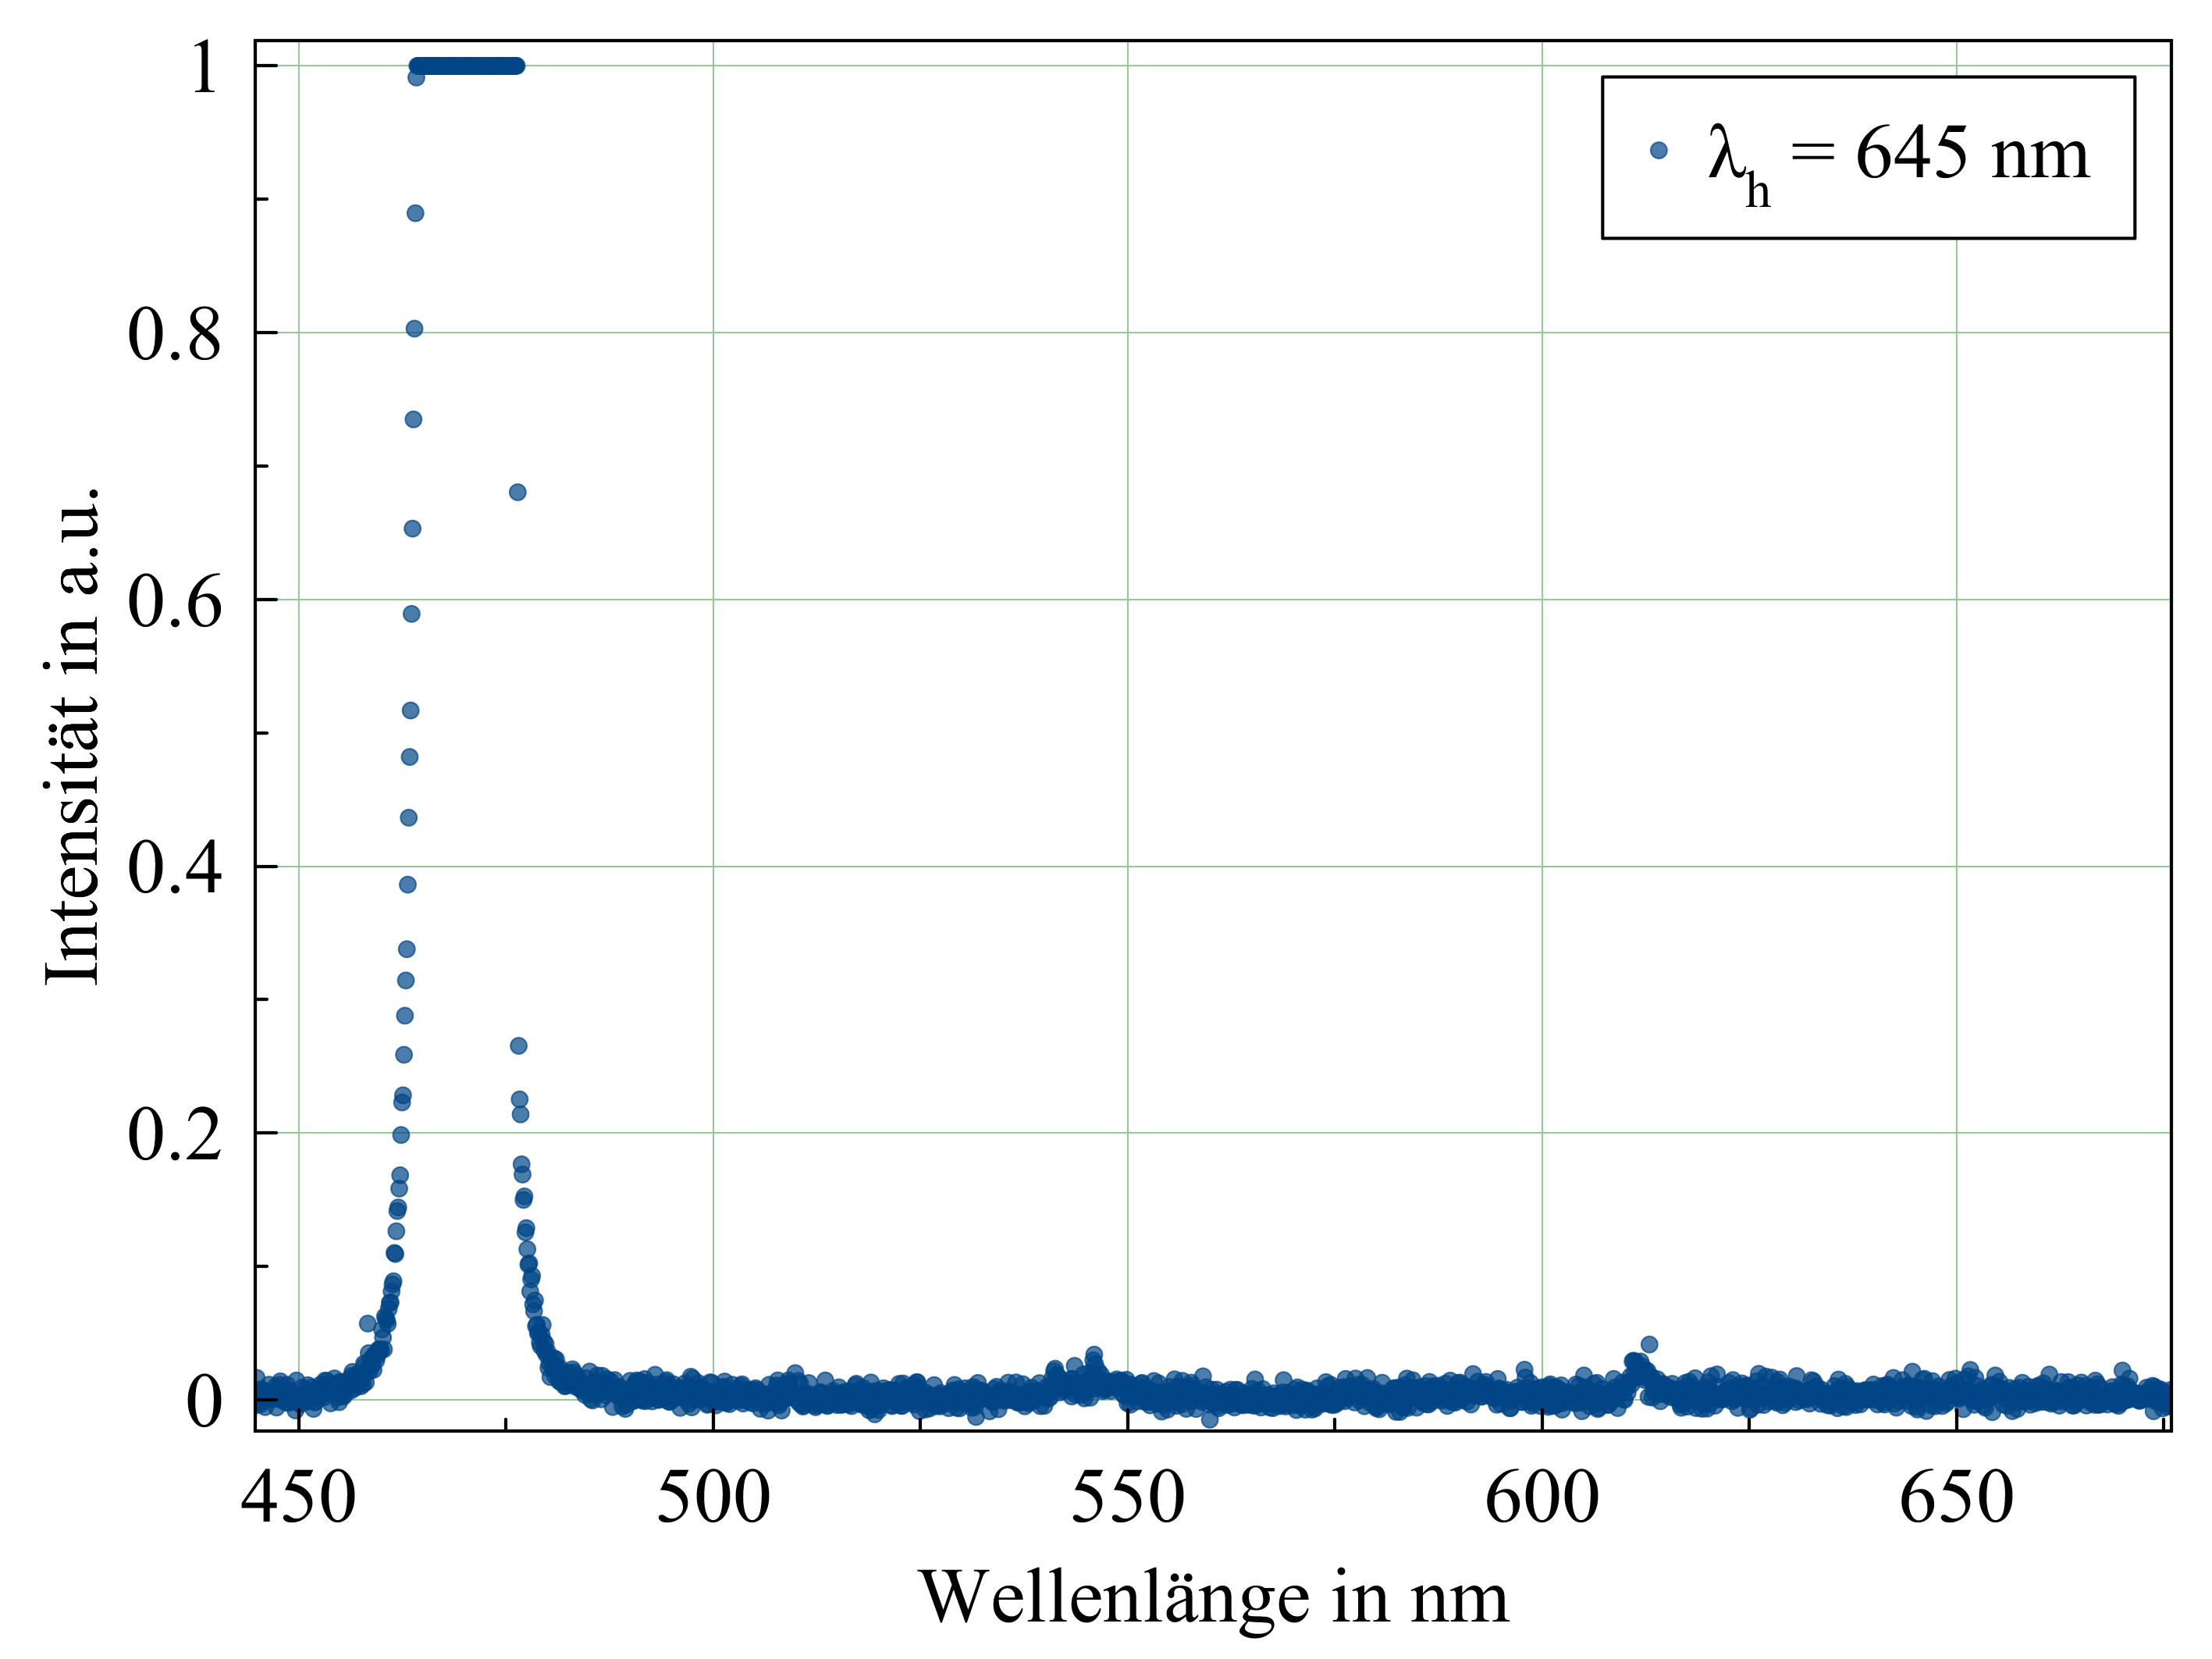
\includegraphics[width=\textwidth]{plots/Weisslicht_645_470.png}
    \caption{$\lambda=\SI{470}{\nano\meter}$}
    \label{fig:PL_645_470}
  \end{subfigure}
  \caption{Photolumineszenzspektrum der $\lambda_h=\SI{645}{\nano\meter}$ Probe.}
  \label{fig:PL_645}
\end{figure}
\begin{figure}[H]
  \centering
  \begin{subfigure}{0.49\textwidth}
    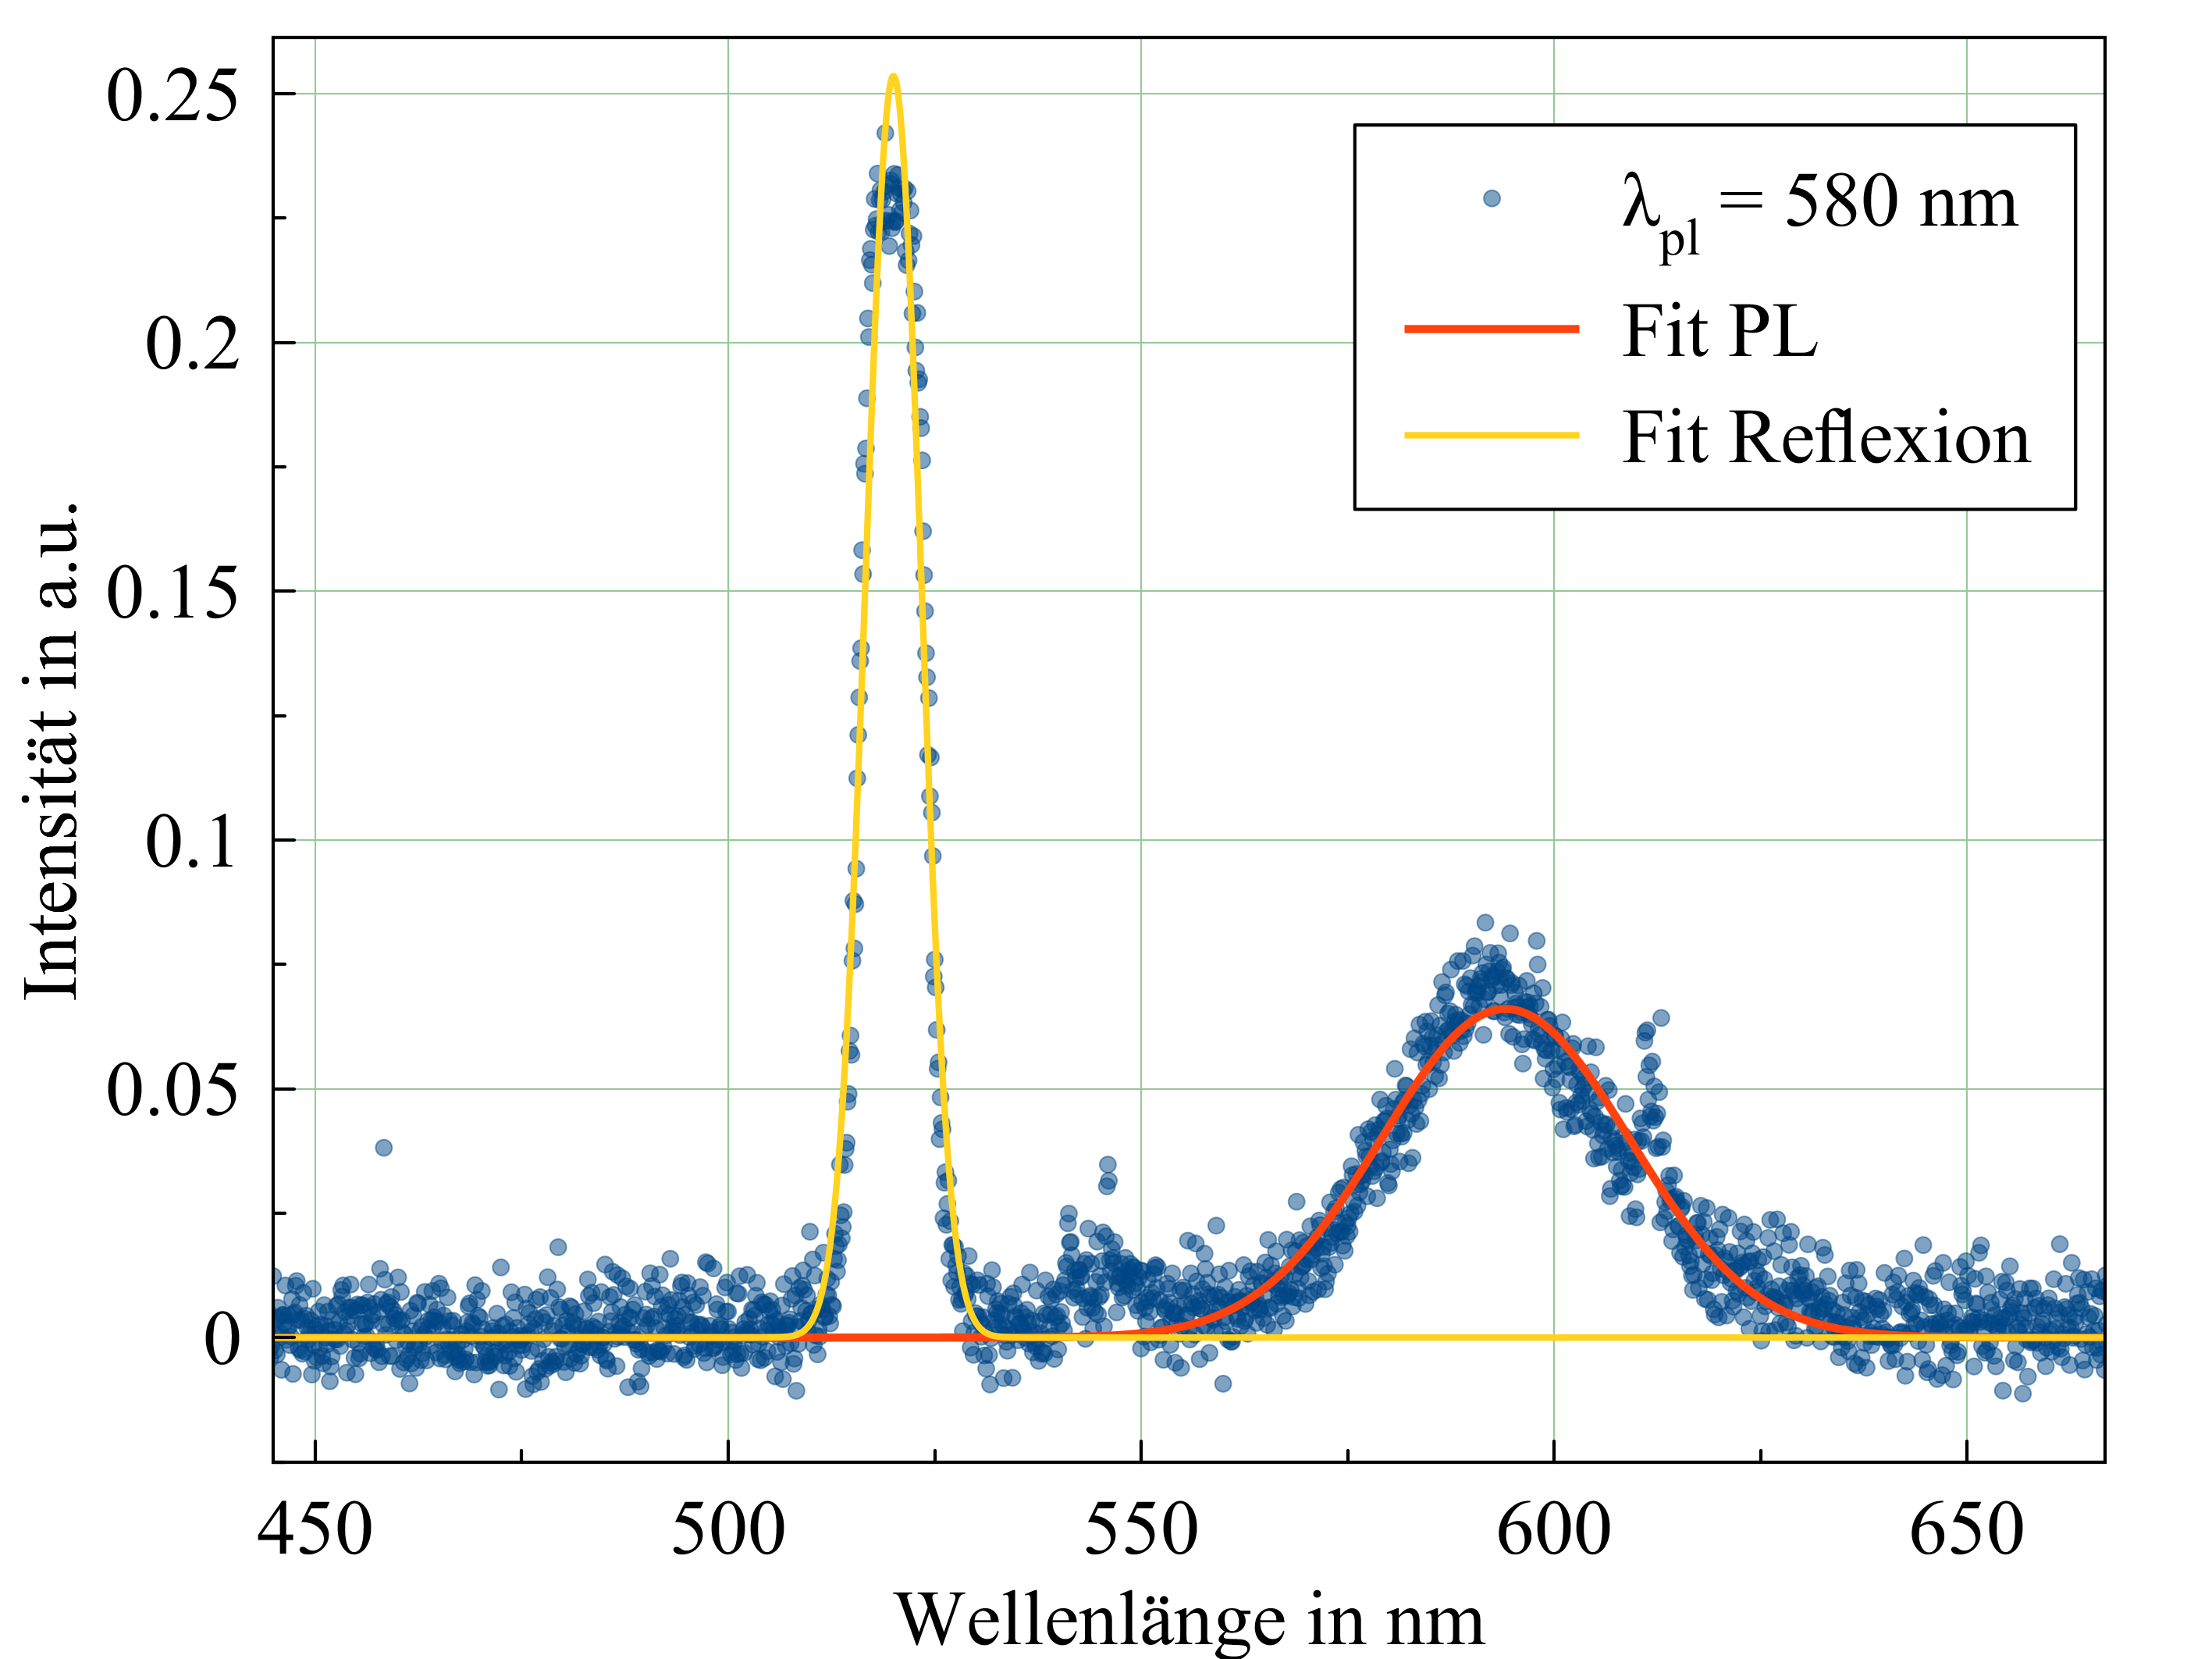
\includegraphics[width=\textwidth]{plots/Weisslicht_580_520.png}
    \caption{$\lambda=\SI{520}{\nano\meter}$}
    \label{fig:PL_580_normus}
  \end{subfigure}
  \begin{subfigure}{0.49\textwidth}
    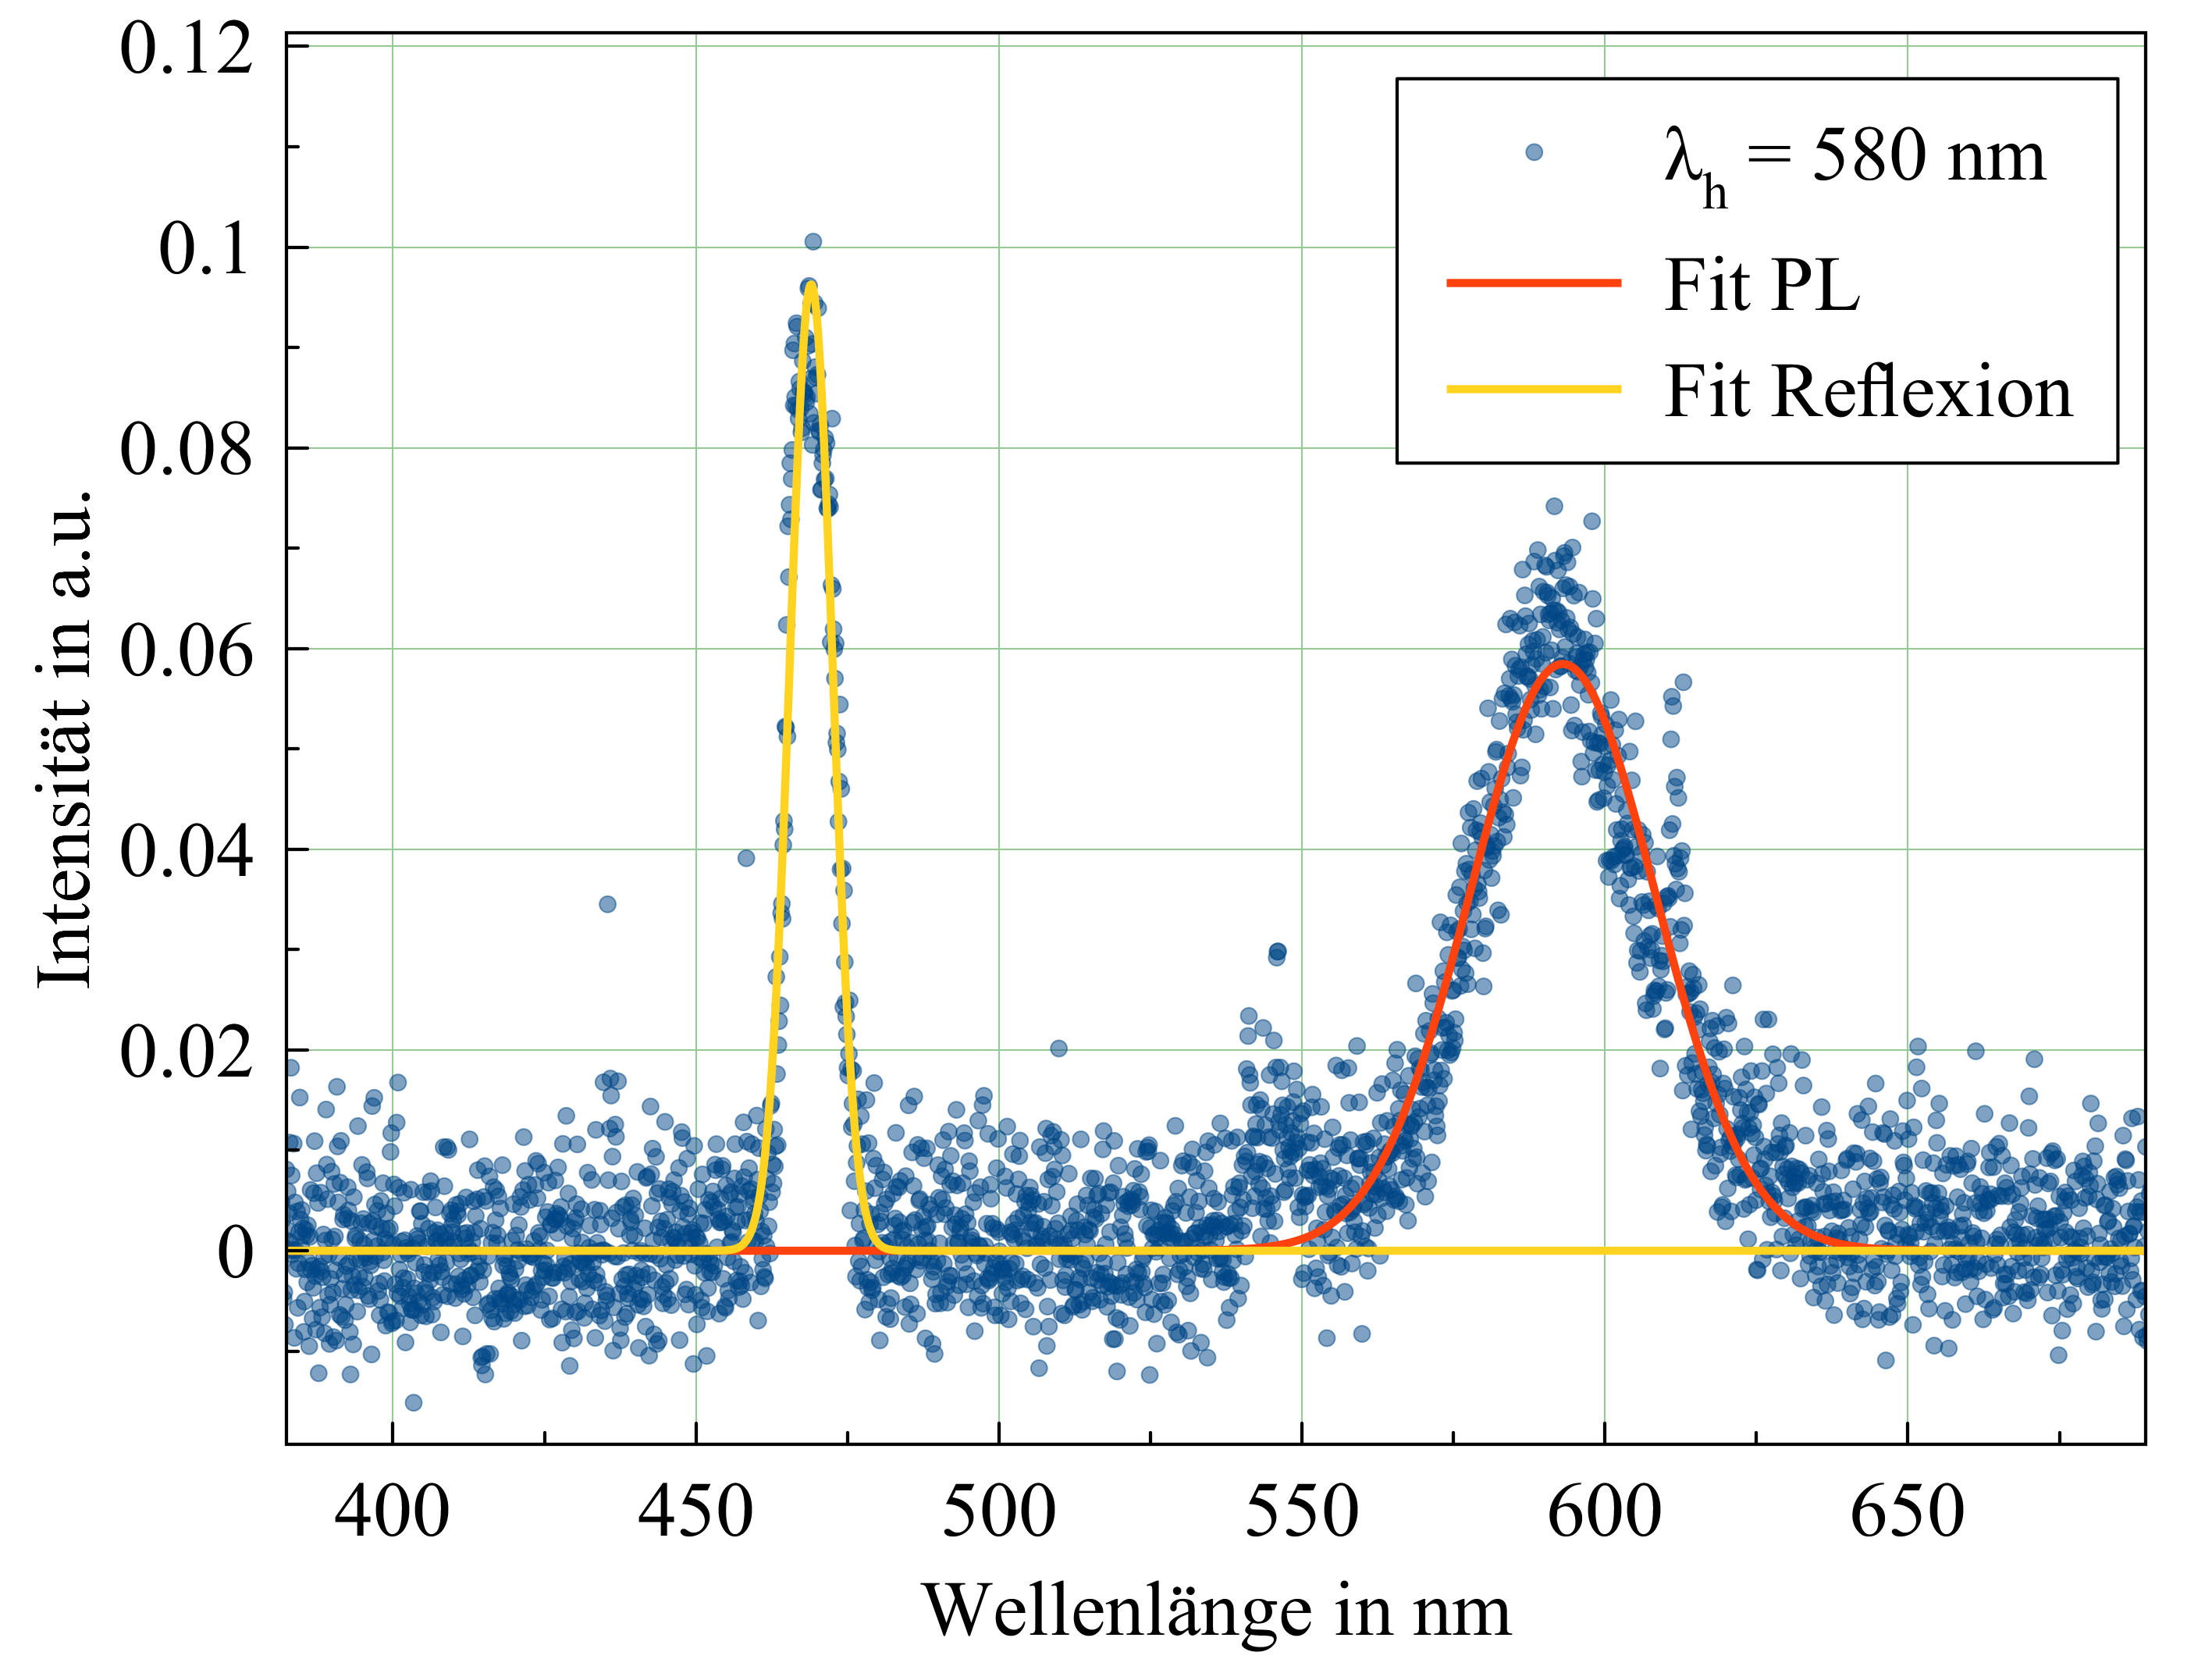
\includegraphics[width=\textwidth]{plots/Weisslicht_580_470.png}
    \caption{$\lambda=\SI{470}{\nano\meter}$}
    \label{fig:PL_580_Satt}
  \end{subfigure}
  \caption{Photolumineszenzspektrum der $\lambda_h=\SI{580}{\nano\meter}$ Probe.}
  \label{fig:PL_580}
\end{figure}
\begin{figure}[H]
  \centering
  \begin{subfigure}{0.49\textwidth}
    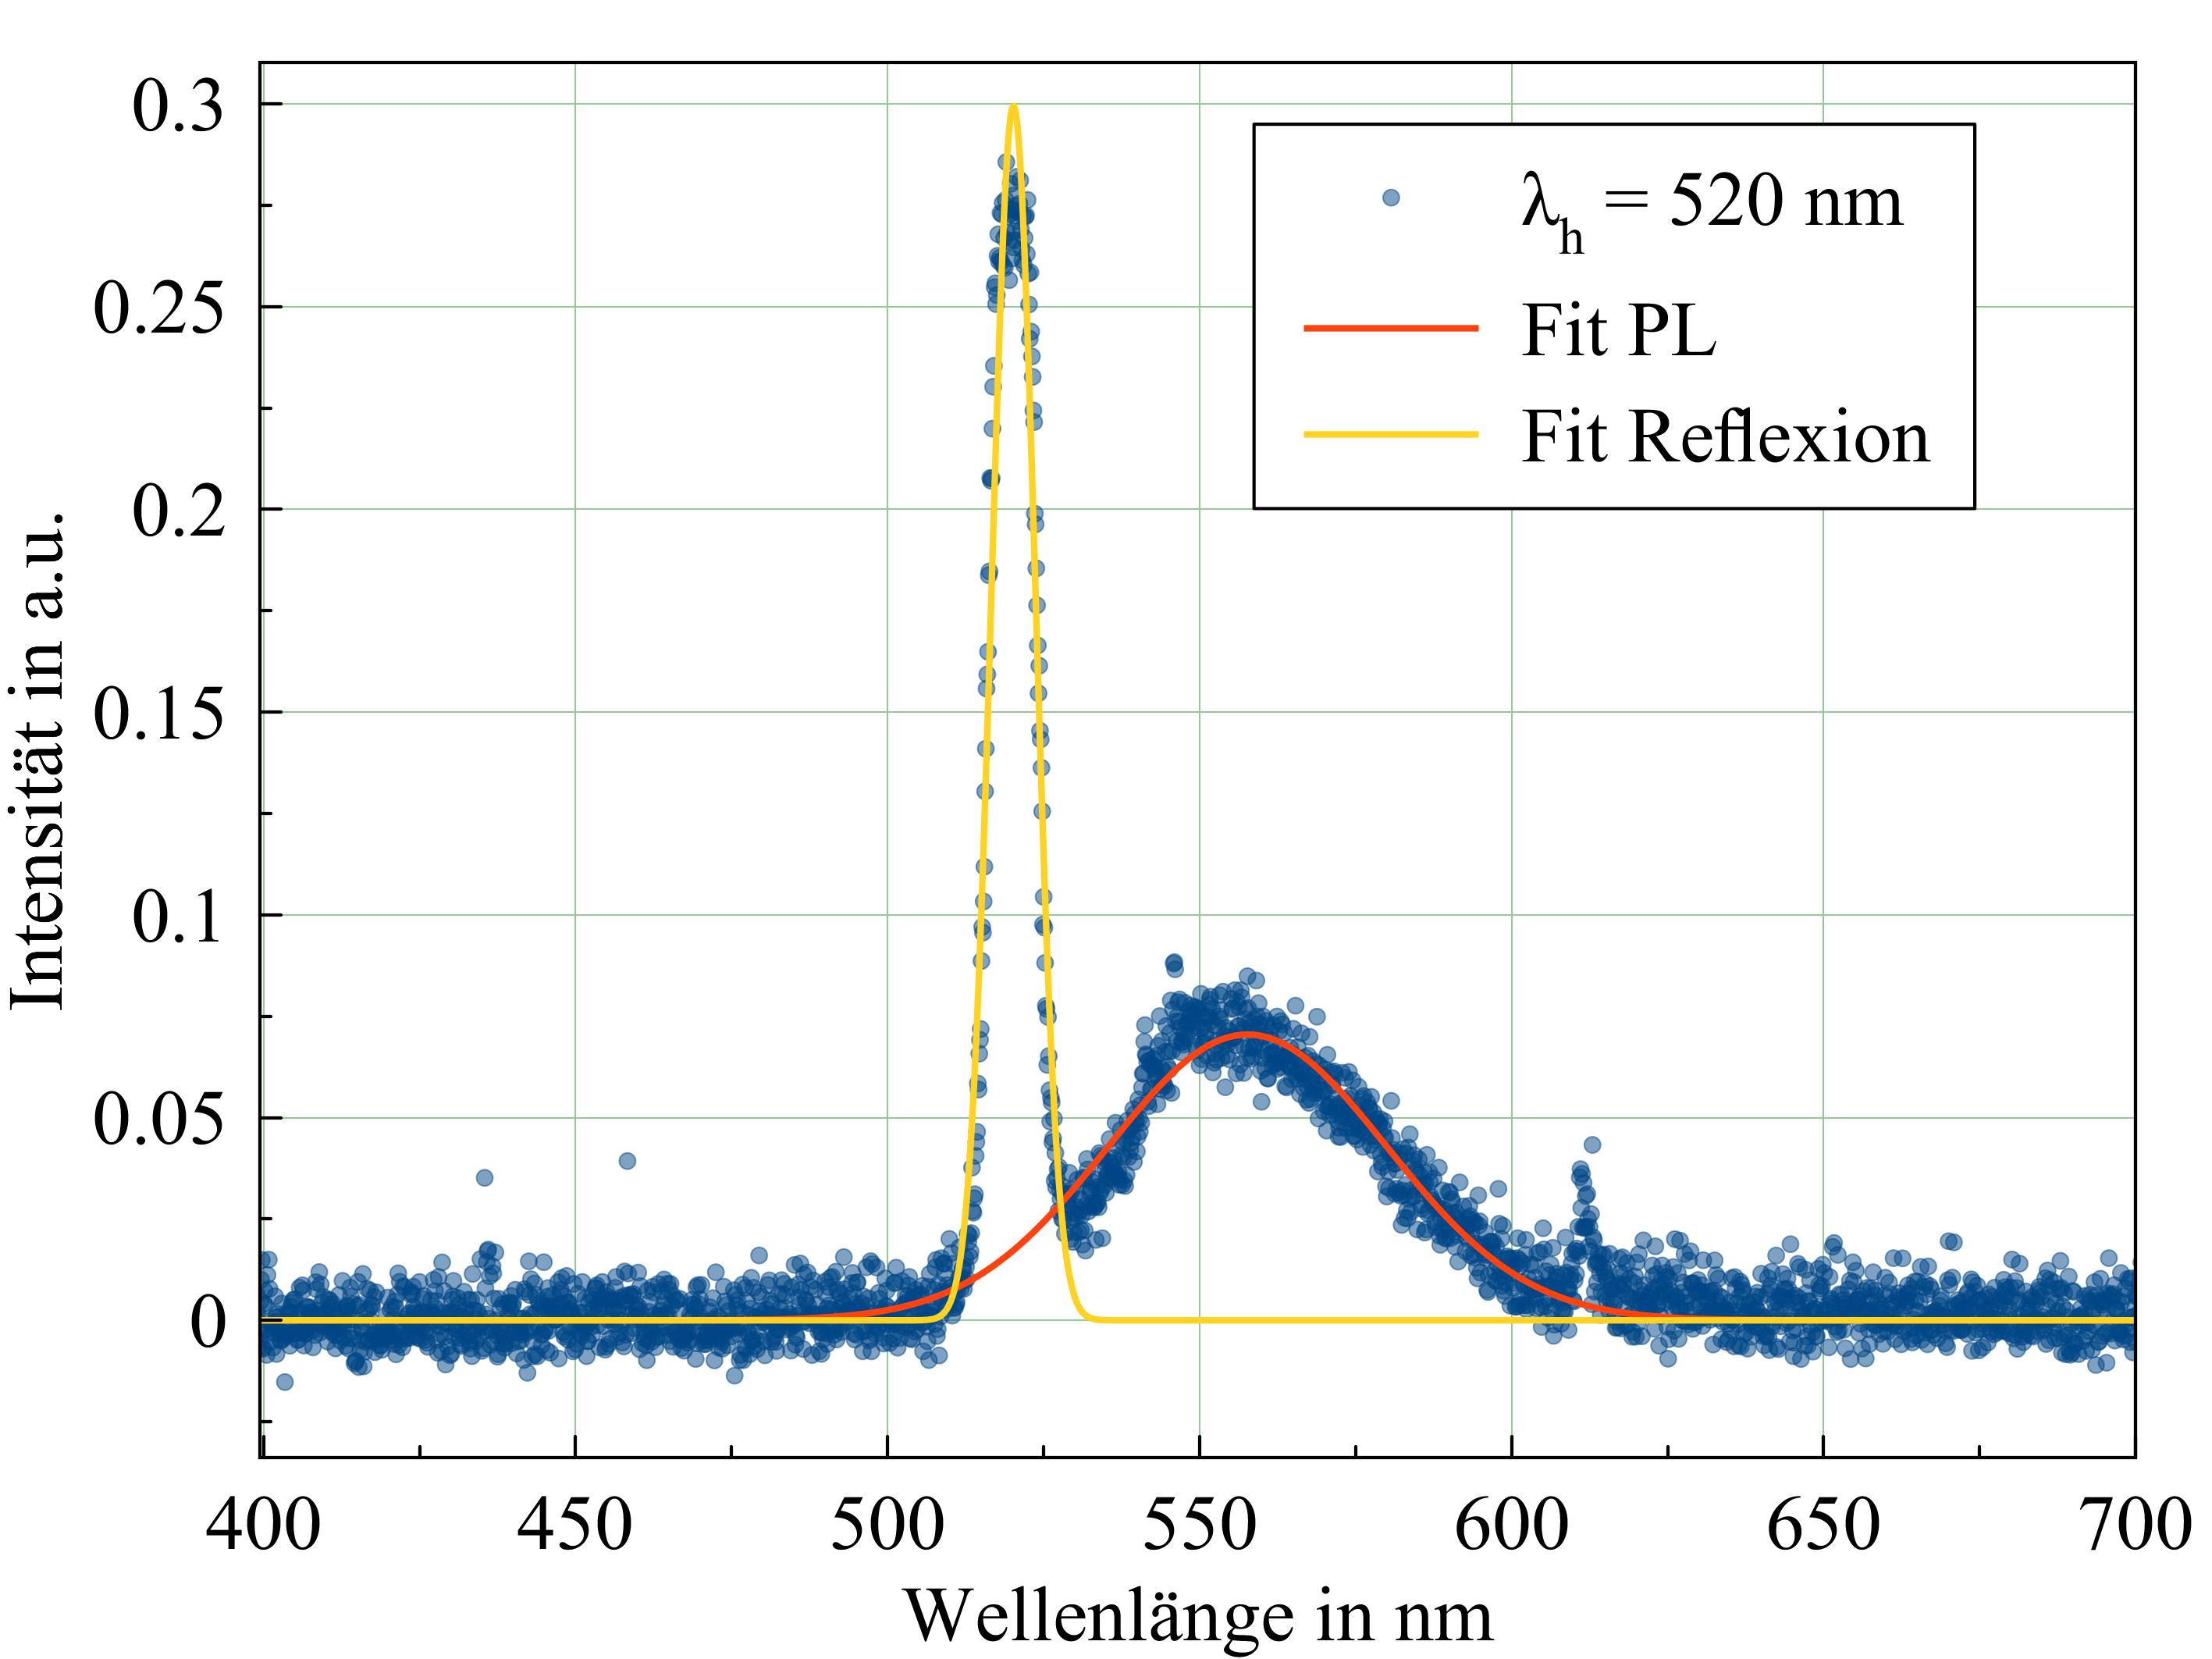
\includegraphics[width=\textwidth]{plots/Weisslicht_520_520.png}
    \caption{$\lambda=\SI{520}{\nano\meter}$}
  \end{subfigure}
  \begin{subfigure}{0.49\textwidth}
    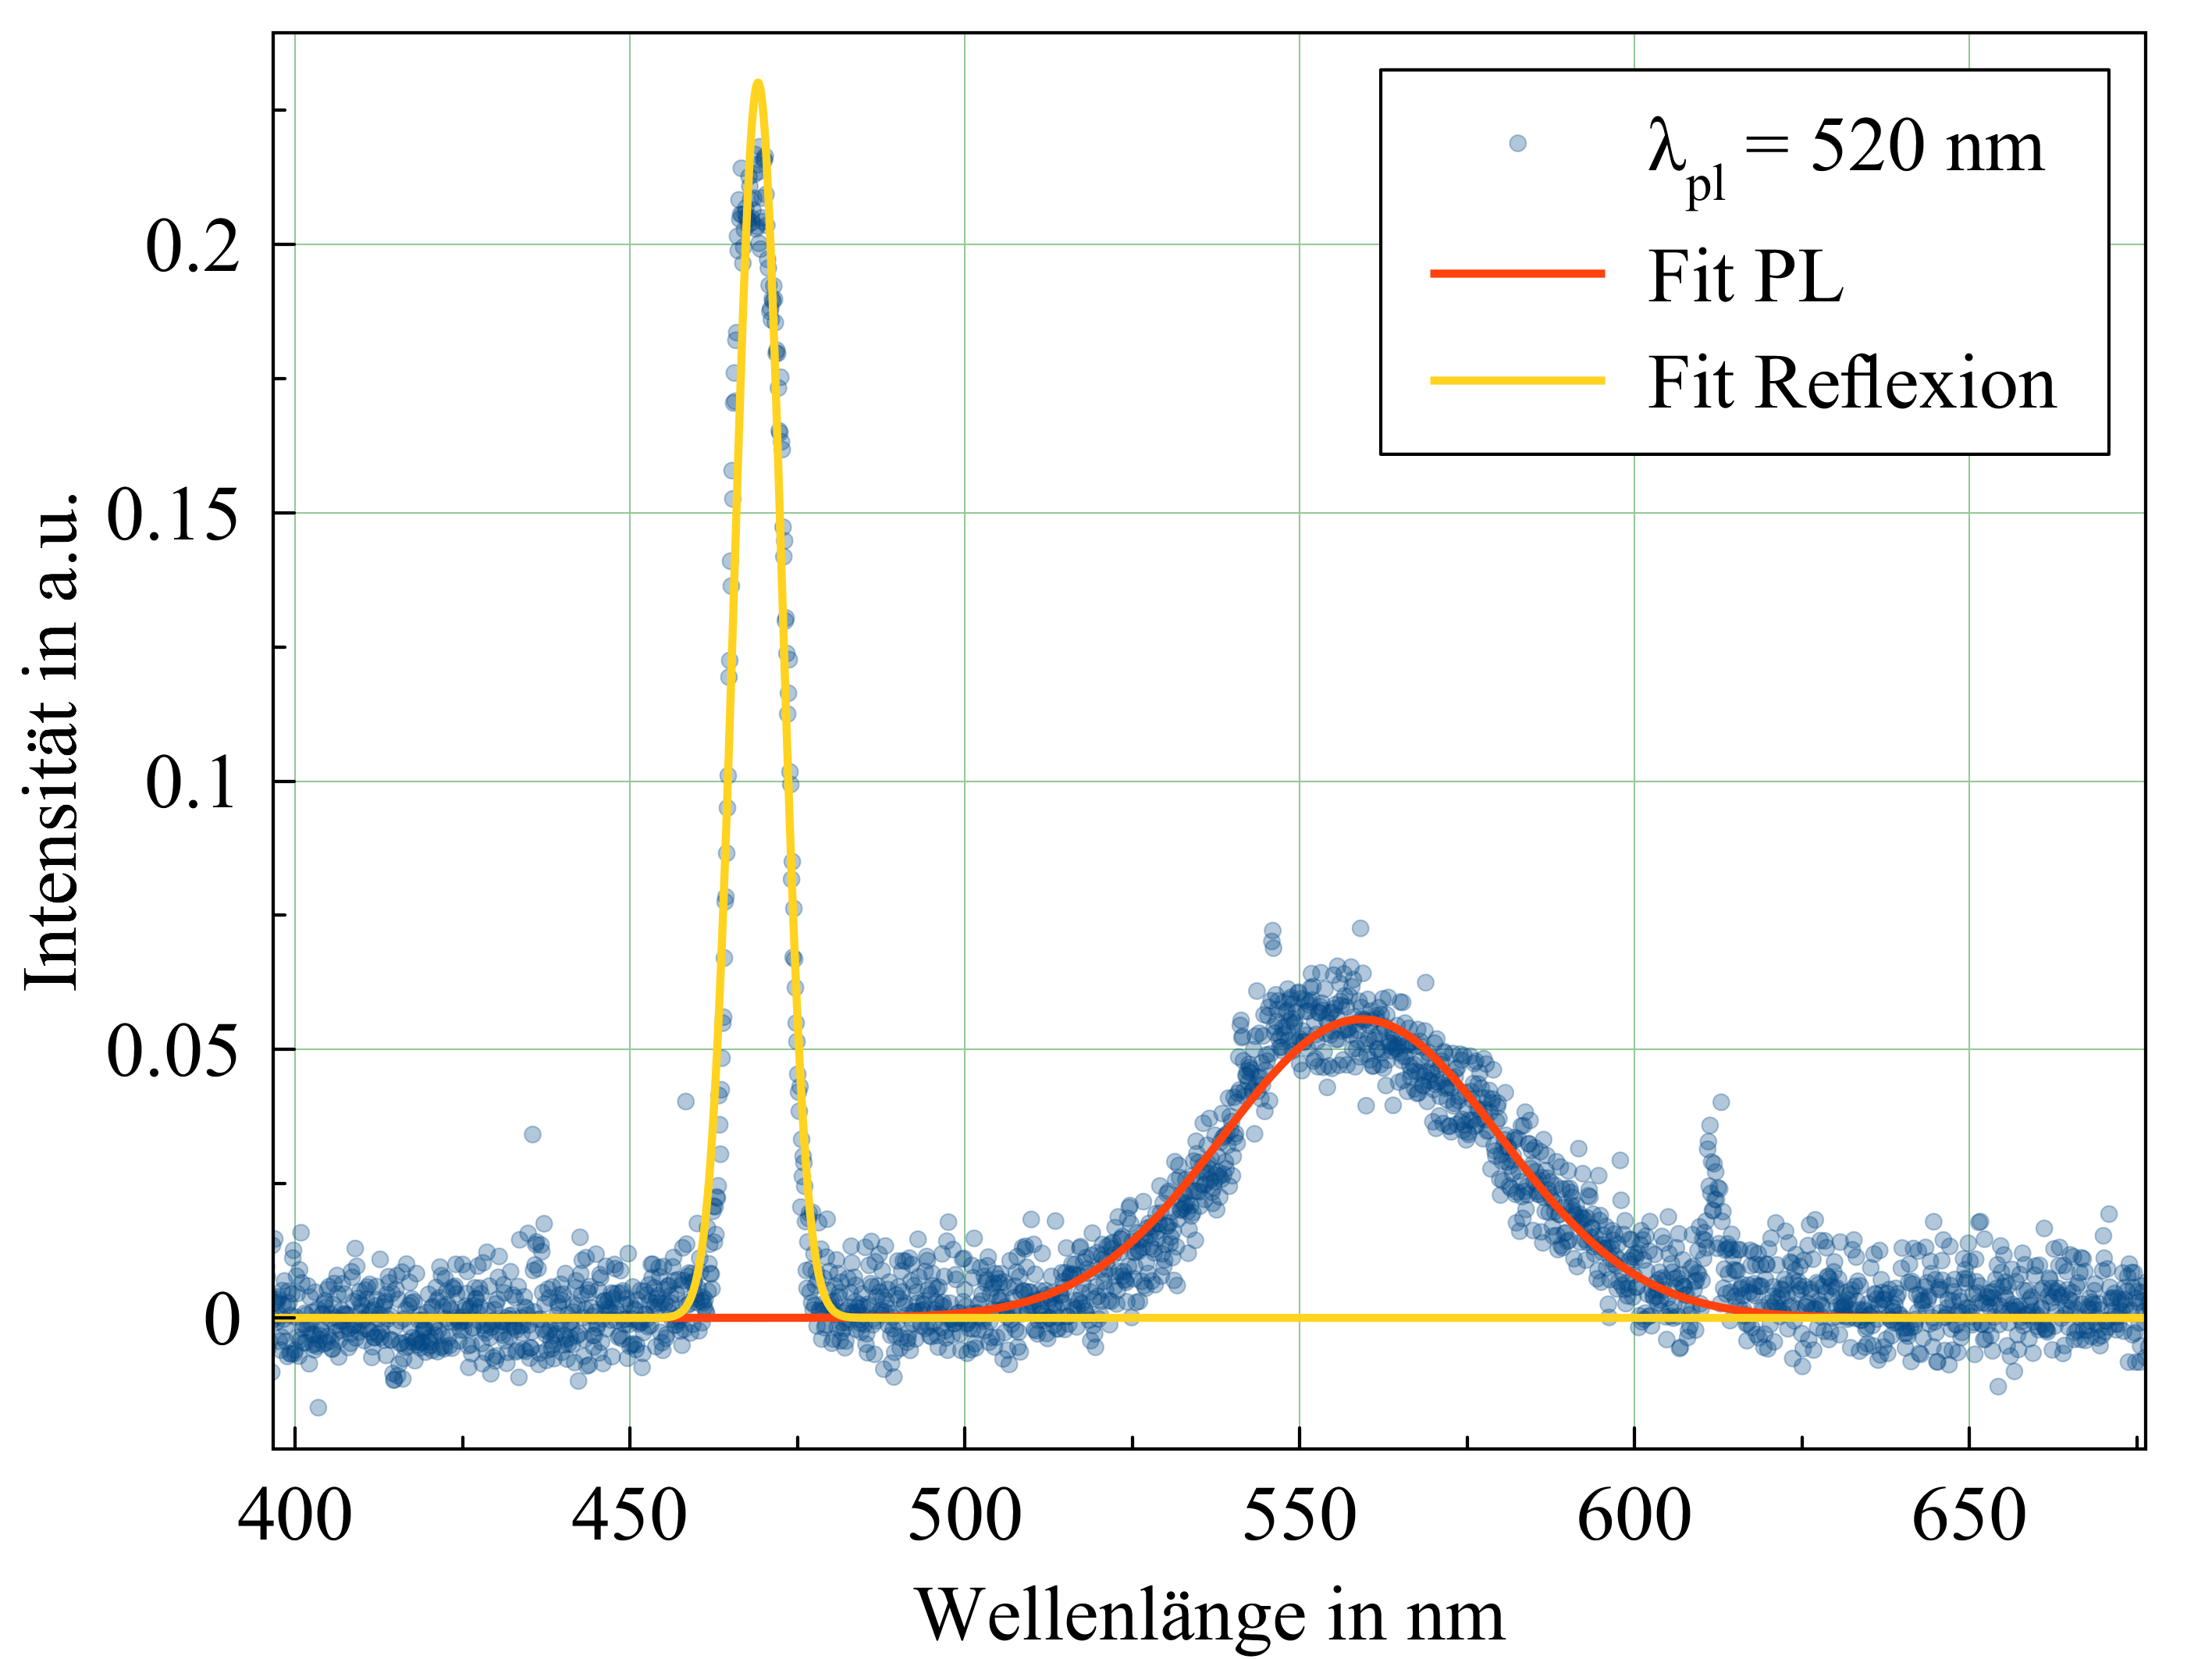
\includegraphics[width=\textwidth]{plots/Weisslicht_520_470.png}
    \caption{$\lambda=\SI{470}{\nano\meter}$}
  \end{subfigure}
  \caption{Photolumineszenzspektrum der $\lambda_h=\SI{520}{\nano\meter}$ Probe.}
  \label{fig:PL_520}
\end{figure}
